\documentclass[11pt]{article}

% --- Standard packages only (no proprietary dependencies) ----------------- %
\usepackage[utf8]{inputenc}
\usepackage[T1]{fontenc}
\usepackage{amsmath,amssymb,amsthm}
\usepackage{graphicx}
\usepackage{booktabs}
\usepackage{multirow}
\usepackage{subcaption}
\usepackage{geometry}
\usepackage{xcolor}
\usepackage{siunitx}
\usepackage[numbers,sort&compress]{natbib}
\usepackage[hidelinks]{hyperref}
\usepackage[capitalise,noabbrev]{cleveref}

\geometry{margin=1in}
\graphicspath{{figures/}}
\sisetup{detect-all}
\emergencystretch=2em  % absorb rare overfull lines gracefully

% --- Theorem-like environments -------------------------------------------- %
\theoremstyle{plain}
\newtheorem{proposition}{Proposition}
\theoremstyle{remark}
\newtheorem{remark}{Remark}

% --- Consistent notation macros ------------------------------------------- %
\newcommand{\R}{\mathbb{R}}
\newcommand{\E}{\mathbb{E}}
\newcommand{\dd}{\,\mathrm{d}}
\newcommand{\Fref}{F_{\mathrm{ref}}}
\newcommand{\Fpref}{F'_{\mathrm{ref}}}
\newcommand{\pref}{p_{\mathrm{ref}}}
\newcommand{\Fhat}{\widehat{F}}
\newcommand{\Fphat}{\widehat{F}'}
\newcommand{\phat}{\widehat{p}}
\newcommand{\Bt}{B_t}
\newcommand{\Ltwo}{L^2}
\newcommand{\xib}{\xi}
\newcommand{\Norm}[1]{\left\lVert #1 \right\rVert}

% --- CSV-derived numbers (generated by scripts/build_report_assets.py) ----- %
% Do not edit by hand; run `make assets` to regenerate. Verified by
% scripts/check_report_numbers.py.
\newcommand{\NRuns}{545}
\newcommand{\NConfigs}{109}
\newcommand{\NSeeds}{5}
\newcommand{\NMethods}{4}
\newcommand{\NSteps}{100{,}000}
\newcommand{\NParticles}{1000}
\newcommand{\BetaVal}{4}
\newcommand{\NFRconfigs}{36}
\newcommand{\AbfIntegF}{15.91}
\newcommand{\AbfFinalF}{0.0137}
\newcommand{\AbfFinalFp}{0.0718}
\newcommand{\AbfBarrier}{4.86\times10^{5}}
\newcommand{\EstIntegF}{14.08}
\newcommand{\EstIntFinalF}{0.0126}
\newcommand{\EstIntGamma}{0.1}
\newcommand{\EstIntBurnin}{0}
\newcommand{\EstIntProb}{60.0}
\newcommand{\EstIntEvt}{1.6\times10^{-5}}
\newcommand{\EstIntegImpPct}{11.5}
\newcommand{\EstFinFinalF}{0.0120}
\newcommand{\EstFinIntegF}{15.25}
\newcommand{\EstFinFinalFp}{0.0673}
\newcommand{\EstFinGamma}{0.01}
\newcommand{\EstFinBurnin}{0.4}
\newcommand{\EstFinProb}{80.0}
\newcommand{\EstFinEvt}{1.1\times10^{-6}}
\newcommand{\EstFinFinalImpPct}{12.5}
\newcommand{\EstFinFinalFpImpPct}{6.3}
\newcommand{\UniIntegF}{14.46}
\newcommand{\UniIntegImpPct}{9.1}
\newcommand{\UniFinalF}{0.0118}
\newcommand{\UniFinFinalImpPct}{13.8}
\newcommand{\OracIntegF}{13.27}
\newcommand{\OracFinalF}{0.0113}
\newcommand{\OracFinalFp}{0.0602}
\newcommand{\OracProb}{100.0}
\newcommand{\OracIntegImpPct}{16.6}
\newcommand{\OracFinalImpPct}{17.3}
\newcommand{\EstOracGapPct}{-6.1}
\newcommand{\EBabfLtwoF}{0.201}
\newcommand{\EBfrLtwoF}{0.098}
\newcommand{\EBgainStrong}{51.3}
\newcommand{\EBcoldWin}{20}
\newcommand{\EBuniGain}{50.5}
\newcommand{\EBoracleGain}{-28.1}
\newcommand{\EBwarmGainBetaFour}{-26.1}
\newcommand{\EBgammaMaxGain}{72.6}
\newcommand{\EBessHi}{101}
\newcommand{\EBessLo}{9}
\newcommand{\WCAabfLtwoF}{0.0835}
\newcommand{\WCAtunedLtwoF}{0.0361}
\newcommand{\WCAtunedGainPct}{55.0}
\newcommand{\WCAtunedWin}{10}
\newcommand{\WCAuniGainPct}{54.6}
\newcommand{\WCAoracleGainPct}{52.7}
\newcommand{\WCAaggrGainPct}{-13.1}
\newcommand{\WCAbudgetLoGain}{35.5}
\newcommand{\WCAbudgetHiGain}{56.9}
\newcommand{\WCAdenseAbfErr}{0.365}
\newcommand{\WCAdenseFrErr}{0.225}


\title{\bfseries Does Fisher--Rao Birth--Death Help Adaptive Biasing Force?\\
A Three-Case Study from a Model Potential to a Condensed-Phase Dimer}
\author{}
\date{\today}

\begin{document}
\maketitle

\begin{abstract}
We study whether augmenting the Adaptive Biasing Force (ABF) method with a
Fisher--Rao (FR) birth--death correction improves the computation of a
reaction-coordinate free energy, and what kind of improvement it can reasonably be
expected to provide. We test this on \emph{three} systems that deliberately probe
different regimes: a two-dimensional double-well \emph{metastability} model with a
quadrature reference; a two-dimensional \emph{entropic-bottleneck} model with a
narrow transverse channel, for which both the reference free energy and the
conditional law $Y\mid X=x\sim\mathcal N(0,1/(\beta\omega(x)^2))$ are analytic;
and a many-body condensed-phase \emph{Weeks--Chandler--Andersen (WCA) dimer} in a
dense solvent, evaluated against a high-accuracy thermodynamic-integration
reference. In each case the FR step reallocates walkers along the reaction
coordinate by killing replicas in over-represented regions and cloning whole
configurations from under-represented regions, nudging the empirical marginal
$\phat_t$ toward a target $q_t$.

The central finding is not a single universal success story, but a regime map. In
the metastability model, where plain ABF already samples reasonably well,
estimated-target FR is a modest accelerator and the oracle diagnostic shows that
target direction can matter. In the cold entropic bottleneck, ABF is starved and
estimated-target FR gives a large gain ($+\EBgainStrong\%$, $\EBcoldWin/20$ seeds),
but the uniform target nearly matches it and the oracle target is worse than ABF;
here density correction and free-energy accuracy are not the same objective. In
the WCA dimer, tuned FR again improves the free energy reliably
($+\WCAtunedGainPct\%$, $\WCAtunedWin/10$ seeds), while the best accuracy occurs
near the edge of an accuracy--diversity tradeoff. Across the cases, FR is best
understood as a marginal-reallocation mechanism whose value depends on how starved
the ABF estimator is, how quickly cloned orthogonal degrees of freedom
re-equilibrate, and how aggressively birth--death erodes ancestor diversity. The
oracle target is therefore a diagnostic control, not a deployable method and not a
universal upper bound.

\end{abstract}

\section{Introduction}
\label{sec:intro}

\subsection{Free-energy computation along a reaction coordinate}
A central task in computational statistical mechanics is to compute the free
energy associated with a low-dimensional \emph{reaction coordinate} of a
high-dimensional system in thermal equilibrium~\citep{LelievreRoussetStoltz2010}.
For most of the development we take a configuration to be a point
$q=(x,y)\in\R^2$\footnote{We write a configuration as $q=(x,y)$ in the
two-dimensional cases; the many-body case of \cref{sec:case_wca} uses
$q\in\R^{2n}$ with a scalar collective variable $z(q)$ in place of $x$
(\cref{rem:manybody}). The symbol $q_t(\cdot)$, always carrying a time subscript
and a scalar argument, denotes instead the Fisher--Rao \emph{target marginal} of
\cref{sec:fr}; the two are never used in the same role.} drawn from the
canonical (Boltzmann--Gibbs) density
\begin{equation}
  \pi(x,y) \;\propto\; e^{-\beta V(x,y)},
  \label{eq:canonical}
\end{equation}
where $V$ is the potential energy and $\beta=1/(k_{\mathrm B}T)$ is the inverse
temperature. Fixing the reaction coordinate to the first coordinate,
$\xib(x,y)=x$, the free energy $F(x)$ and the local mean force $F'(x)$ along
$\xib$ are the objects of interest. The difficulty is metastability: when $V$
has well-separated basins along $x$, unbiased Langevin dynamics crosses the
barrier rarely, so a direct estimate of $F$ converges intolerably slowly.

\subsection{Adaptive Biasing Force}
The Adaptive Biasing Force (ABF) method~\citep{DarvePohorille2001,Henin2004,
Comer2015} removes this metastability adaptively. It maintains a running
estimate $\Fphat_t(x)$ of the mean force and applies the antiderivative
$\Bt(x)=\int^x\Fphat_t$ as a bias that depends only on $x$. As
$\Bt\to F$, the effective dynamics along $x$ becomes diffusive and the
reaction coordinate is explored freely, while --- crucially --- the bias does
not change the conditional law of the orthogonal degrees of freedom given $x$.
ABF is mathematically well understood, with long-time convergence
guarantees~\citep{LelievreRoussetStoltz2008}, and is a natural baseline against
which to measure any proposed enhancement.

\subsection{Why add a Fisher--Rao correction?}
ABF accelerates exploration through the \emph{force}, but it does not directly
control \emph{where the particles are}. Early in a simulation the estimated bias
is poor, so the empirical reaction-coordinate marginal $\phat_t(x)$ can remain
concentrated in the initial basin, starving other values of $x$ of the samples
ABF needs to estimate $F'(x)$ there. A Fisher--Rao (FR) birth--death
correction~\citep{LuLuNolen2019} addresses exactly this: interpreting the
evolution of $\phat_t$ as a gradient flow of relative entropy in the
Fisher--Rao geometry~\citep{Amari2016}, one reallocates probability mass by
\emph{killing} particles in over-represented regions and \emph{cloning}
particles in under-represented regions, driving $\phat_t$ toward a chosen target
marginal $q_t(x)$ without integrating any additional dynamics. Coupling such a
correction to ABF is appealing because the two act on complementary objects
(force versus density), but it is not automatically beneficial: a birth--death
step resamples \emph{whole} configurations $(x,y)$, and if it distorts the
conditional law $Y\mid X=x$ it will corrupt precisely the quantity ABF estimates.

\subsection{Central question and contributions}
This report asks how FR changes ABF across \emph{three} controlled systems, not
whether one slogan can describe all of them:
\begin{enumerate}
  \item \textbf{When does marginal reallocation help ABF, and when can it hurt?}
        (Q1)
  \item \textbf{What target and rate choices make FR useful in each regime?}
        (Q2--Q3)
  \item \textbf{What limitations and failure modes appear when the system becomes
        more realistic?} (Q4)
\end{enumerate}
The systems are (i) a two-dimensional double-well \emph{metastability} model
with a quadrature reference (\cref{sec:case_meta}); (ii) a two-dimensional
\emph{entropic-bottleneck} model with a narrow transverse channel, for which both
the reference free energy \emph{and} the conditional law $Y\mid X=x$ are analytic
(\cref{sec:case_eb}); and (iii) a many-body \emph{Weeks--Chandler--Andersen
(WCA) dimer} in a dense solvent with a high-accuracy thermodynamic-integration
reference (\cref{sec:case_wca}). Together they span three regimes: an easy
baseline where target direction can matter, a cold analytic bottleneck where
density correction and free-energy accuracy can come apart, and a many-body
system where improved coverage must be balanced against loss of lineage diversity.

Our contributions are: (i) a consistent ABF--FR notation that covers both the
analytic two-dimensional models and the many-body WCA collective variable
(\cref{sec:abf,sec:fr}); (ii) three matched-seed production studies that quantify
both the practical estimated-target method and diagnostic uniform/oracle targets
(\cref{sec:case_meta,sec:case_eb,sec:case_wca}); and (iii) a cross-case synthesis
(\cref{sec:synthesis}) that explains why the conclusions are intentionally
different across examples. A recurring methodological point is the careful
interpretation of an \emph{oracle} target that uses the reference free energy: it
is a diagnostic control, never a deployable method and not a universal upper
bound. Its behaviour is itself part of the evidence: best in the easy
metastability setting, approximately tied with the practical target in WCA, and
worse than ABF in the cold entropic bottleneck.

\section{Background: ABF for a reaction-coordinate free energy}
\label{sec:abf}

\subsection{Free energy and the unbiased marginal}
With reaction coordinate $\xib(x,y)=x$, the unbiased reaction-coordinate
marginal of the canonical density~\eqref{eq:canonical} is
\begin{equation}
  \pref(x) \;=\;
  \frac{\displaystyle\int e^{-\beta V(x,y)}\dd y}
       {\displaystyle\iint e^{-\beta V(x,y)}\dd x\dd y},
  \label{eq:pref}
\end{equation}
and the free energy along $\xib$ is, up to an additive constant,
\begin{equation}
  \Fref(x) \;=\; -\frac{1}{\beta}\,\log \pref(x) + C.
  \label{eq:Fref}
\end{equation}
Because $F$ is defined only up to the constant $C$, every free-energy profile in
this report --- both estimates and the reference --- is \emph{centred} (its mean
over the interior evaluation window is subtracted) before any $\Ltwo$ error is
formed; otherwise a meaningless constant offset would dominate the comparison.
The reference quantities are computed by a one-dimensional $y$-quadrature on a
fine grid with a log-sum-exp shift for numerical stability, which is exact up to
discretisation and provides the ground truth $\Fref,\Fpref,\pref$.

\subsection{The mean force is the object ABF estimates}
Differentiating~\eqref{eq:Fref} and using $\partial_x \pref$ gives the
\emph{mean force}
\begin{equation}
  \Fpref(x) \;=\;
  \frac{\displaystyle\int \partial_x V(x,y)\,e^{-\beta V(x,y)}\dd y}
       {\displaystyle\int e^{-\beta V(x,y)}\dd y}
  \;=\; \E_{\pi}\!\left[\,\partial_x V(X,Y)\,\middle|\, X=x\,\right].
  \label{eq:meanforce}
\end{equation}
Equation~\eqref{eq:meanforce} is the cornerstone of ABF: the gradient of the
free energy equals the \emph{conditional expectation of the instantaneous force}
$\partial_x V$ given the reaction coordinate. It is a local, sample-based
quantity --- no integral of $V$ is required --- so it can be estimated on the
fly from the particles currently at $X\approx x$, and the free energy is then
recovered by quadrature, $\Fhat(x)=\int^x \Fphat$.

\subsection{Biased dynamics}
ABF simulates $N$ overdamped Langevin replicas that share one running mean-force
estimate $\Fphat_t(x)\approx\Fpref(x)$ with bias potential
$\Bt(x)=\int^x\Fphat_t$. Each replica $(X_t,Y_t)$ evolves as
\begin{equation}
  \begin{aligned}
    \dd X_t &= \bigl[-\partial_x V(X_t,Y_t) + \Fphat_t(X_t)\bigr]\dd t
              + \sqrt{2/\beta}\,\dd W_t^x, \\
    \dd Y_t &= -\,\partial_y V(X_t,Y_t)\,\dd t
              + \sqrt{2/\beta}\,\dd W_t^y,
  \end{aligned}
  \label{eq:abf_sde}
\end{equation}
with independent Brownian motions $W^x,W^y$. The added force $+\Fphat_t(X_t)$
acts \emph{only} in the $x$-direction; the $y$-dynamics is unbiased. When
$\Fphat_t\to\Fpref$ the net drift along $x$ becomes $-\partial_x(V-F)$, whose
$x$-marginal equilibrium is flat, so the reaction coordinate diffuses freely
across the barrier.

\subsection{Why the bias does not spoil the mean-force estimate}
A bias that depends only on $x$ leaves the conditional law of $Y$ given $X=x$
invariant. This is what makes ABF self-consistent.

\begin{proposition}[Conditional invariance under an $x$-only bias]
\label{prop:cond_invariance}
Let $\nu$ be the canonical measure $\nu\propto e^{-\beta V(x,y)}$ and let
$\nu_B\propto e^{-\beta\,[V(x,y)-B(x)]}$ be the measure biased by any function
$B$ of $x$ alone. Then for every $x$ the conditionals coincide,
$\nu_B(y\mid X=x)=\nu(y\mid X=x)$, and consequently
\begin{equation}
  \E_{\nu_B}\!\left[\partial_x V(X,Y)\mid X=x\right]
  \;=\;
  \E_{\nu}\!\left[\partial_x V(X,Y)\mid X=x\right]
  \;=\; \Fpref(x).
  \label{eq:cond_equal}
\end{equation}
\end{proposition}

\begin{proof}
At fixed $X=x$ the bias factor $e^{\beta B(x)}$ is a constant in $y$ and cancels
between numerator and normaliser of the conditional density:
\[
  \nu_B(y\mid X=x)
  = \frac{e^{-\beta[V(x,y)-B(x)]}}{\int e^{-\beta[V(x,y')-B(x)]}\dd y'}
  = \frac{e^{-\beta V(x,y)}}{\int e^{-\beta V(x,y')}\dd y'}
  = \nu(y\mid X=x).
\]
Taking the conditional expectation of $\partial_x V$ under this common
conditional gives~\eqref{eq:cond_equal}, the last equality
being~\eqref{eq:meanforce}.
\end{proof}

\Cref{prop:cond_invariance} is the reason ABF works: even though the biased
ensemble~\eqref{eq:abf_sde} has a different $x$-marginal than the canonical
one, the conditional samples $Y\mid X=x$ remain canonical, so the empirical
conditional average of $\partial_x V$ is an unbiased target for
$\Fpref(x)$. Any modification of ABF must respect this property; in particular,
a birth--death correction that resamples whole configurations $(x,y)$ is
only admissible if it too leaves $Y\mid X=x$ (approximately) intact ---
a hypothesis we test directly in each of the three case studies
(\cref{sec:case_meta,sec:case_eb,sec:case_wca}).

\begin{remark}[Generalisation to many-body systems]
\label{rem:manybody}
Two of our three systems are two-dimensional with $\xib=x$, but the WCA dimer of
\cref{sec:case_wca} is a many-body system: a configuration is the full vector
$q\in\R^{2n}$ of all particle coordinates, and the reaction coordinate is a
scalar \emph{collective variable} $z(q)$ (a scaled bond length) rather than a
single Cartesian component. \Cref{prop:cond_invariance} holds verbatim under the
substitution $x\mapsto z(q)$ and $y\mapsto$ the orthogonal complement of $z$ on
the constant-$z$ manifold (here the solvent coordinates and the transverse dimer
modes): a bias $B(z)$ that depends on the collective variable alone is constant
on each level set of $z$, so it cancels in the conditional density and leaves the
law of all orthogonal degrees of freedom invariant. Consequently the mean force
along $z$ --- which for a nonlinear $z(q)$ also carries a geometric term
(\cref{sec:case_wca}) --- is still estimated without bias. The only requirement
the FR step must meet is the same one as in two dimensions: a clone must copy the
\emph{entire} configuration $q\in\R^{2n}$, so that the orthogonal coordinates
travel with $z$ and the conditional law is preserved.
\end{remark}

\subsection{The ABF mean-force estimator}
\label{sec:abf_estimator}
In the kernel form used by the reference implementation, $\Fphat$ is a
Nadaraya--Watson running average of the instantaneous force,
\begin{equation}
  \Fphat_n(x) \;=\;
  \frac{\sum_{k\le n}\sum_i K_h(x-X_k^i)\,\partial_x V(X_k^i,Y_k^i)}
       {\sum_{k\le n}\sum_i K_h(x-X_k^i)},
  \label{eq:nw}
\end{equation}
with a Gaussian kernel $K_h$ of bandwidth $h$, accumulated over all replicas
$i$ and past steps $k$; the free-energy estimate is its pinned trapezoidal
antiderivative, $\Fhat_n(x)=\int_0^x\Fphat_n$, and we use $\Bt\equiv\Fhat$ as
the bias. The GPU backend used for the production study replaces the
$O(n_{\mathrm{grid}}\,N)$ kernel sums by an $O(N+n_{\mathrm{grid}})$
\emph{binned-smoothed} estimator: particles are scattered onto the $x$-grid and
the count and force histograms are Gaussian-smoothed, so that
$\Fphat(x)=\mathrm{smooth(force)}/\mathrm{smooth(count)}$ is a Riemann-sum
approximation of~\eqref{eq:nw} that converges to it as the grid spacing
vanishes. The two estimators are validated to agree to well under $1\%$ on
static tests (\cref{sec:design}).

\section{The Fisher--Rao marginal correction}
\label{sec:fr}

The Fisher--Rao (FR) correction is a birth--death / particle-reallocation step
that acts on the \emph{reaction-coordinate marginal} of the ensemble. It is
interleaved with the ABF dynamics~\eqref{eq:abf_sde} and is designed to drive the
empirical marginal $\phat_t(x)$ toward a target marginal $q_t(x)$, without
adding any drift to the $(x,y)$ dynamics.

\subsection{Empirical and target marginals}
At step $n$, after the Langevin proposal of all $N$ replicas, the empirical
reaction-coordinate marginal is estimated by a (reflected, edge-corrected)
kernel density / binned-smoothed estimate of bandwidth $\eta$,
\begin{equation}
  \phat_{n}(x) \;=\; \frac{1}{N}\sum_{i=1}^{N} K_\eta\!\bigl(x-X_n^i\bigr),
  \label{eq:phat}
\end{equation}
renormalised on the $x$-grid. The target $q_n(x)$ is one of three choices
(\cref{sec:targets}); all are nonnegative and normalised, $\int q_n=1$.

\subsection{Fisher--Rao score}
For each particle the FR \emph{score} is the pointwise log-ratio of the
empirical to the target marginal, with its ensemble mean removed:
\begin{equation}
  S_i \;=\;
  \log\frac{\phat_n(X^i_n)+\varepsilon}{q_n(X^i_n)+\varepsilon}
  \;-\;
  \underbrace{\int \phat_n(z)\,\log\frac{\phat_n(z)}{q_n(z)}\dd z}
  _{=\,\mathrm{KL}(\phat_n\,\Vert\,q_n)} ,
  \label{eq:score}
\end{equation}
where $\varepsilon>0$ is a small regulariser and the integral baseline equals
the Kullback--Leibler divergence $\mathrm{KL}(\phat_n\Vert q_n)$ (a grid
quadrature; it coincides with the Monte-Carlo baseline
$\tfrac1N\sum_k\log[\phat_n(X^k)/q_n(X^k)]$ up to discretisation). Subtracting
the baseline makes the score mean-zero, so the birth--death step below conserves
the expected particle number. The score is clipped to $[-S_{\max},S_{\max}]$
for stability. Its interpretation is direct:
\begin{itemize}
  \item $S_i>0$: $X^i$ lies where $\phat_n>q_n$, an \emph{over-represented}
        region (too many particles);
  \item $S_i<0$: $X^i$ lies where $\phat_n<q_n$, an \emph{under-represented}
        region (too few particles).
\end{itemize}

\subsection{Birth--death resampling}
The FR step approximates the Fisher--Rao gradient flow of
$\mathrm{KL}(\phat\Vert q)$ as a fixed-$N$ particle reallocation. Over a sub-step
of length $\Delta t$ and at effective rate $\gamma_n^{\mathrm{eff}}$
(\cref{sec:schedule}), each \emph{over-represented} particle ($S_i>0$) is marked
for death with probability
\begin{equation}
  \mathbb P(\text{$i$ dies}) \;=\; 1-\exp\!\bigl(-\gamma_n^{\mathrm{eff}}\,S_i\,\Delta t\bigr),
  \label{eq:death}
\end{equation}
and particles with $S_i<0$ supply clone sources. The WCA and metastability
backends implement this in the direct death-replacement form: killed slots are
filled by clones sampled from the under-represented pool, with weights increasing
with $|S_i|$. The entropic-bottleneck backend uses a vectorised but closely
related fixed-$N$ survivor/clone-pool variant. This distinction matters for exact
diagnostics, but not for the mechanism studied here: all variants move mass along
the reaction coordinate by copying whole configurations from under-represented
regions into over-represented ones.

Cloning copies the \emph{whole} configuration $(X^i,Y^i)$ --- the score depends
only on $x$, but the $y$-coordinate must travel with its $x$-coordinate, or
\cref{prop:cond_invariance} would be violated. The step is made deliberately
gentle by three safeguards: (i) a burn-in and soft ramp on the rate; (ii) score
clipping to $[-S_{\max},S_{\max}]$; and (iii) a hard cap $f_{\max}$ on the
fraction of particles replaced per event (\texttt{max\_event\_fraction}). The
numerical values of $S_{\max}$, $f_{\max}$ and the FR stride
\texttt{fr\_every} are case-specific and are listed in each case's design table.

\subsection{Notation across cases}
\label{sec:fr_notation}
The same FR principle is applied to all three systems, but the implementation and
two parameter names differ slightly across backends. The birth--death \emph{rate}
is written $\gamma$ in the analytic two-dimensional cases
(\cref{sec:case_meta,sec:case_eb}) and \texttt{fr\_rate} in WCA
(\cref{sec:case_wca}); they play the same role in~\eqref{eq:death}. The
\emph{onset} of FR is parameterised as a burn-in \emph{fraction} $b$ in the
analytic cases (\eqref{eq:ramp}, $n_{\mathrm{burnin}}=\lfloor b\,
n_{\mathrm{steps}}\rfloor$) and as an absolute step count
\texttt{fr\_start\_steps} in WCA; the two are related by
$b\approx\texttt{fr\_start\_steps}/n_{\mathrm{steps}}$. Where a case uses a
collective variable $z(q)$ rather than $x$, read $x\mapsto z$ throughout this
section (\cref{rem:manybody}).

\subsection{Rate schedule}
\label{sec:schedule}
The FR rate is zero during an initial burn-in of $n_{\mathrm{burnin}}=
\lfloor b\,n_{\mathrm{steps}}\rfloor$ steps (burn-in fraction $b$), then ramps
softly to its maximum $\gamma$,
\begin{equation}
  \gamma_n^{\mathrm{eff}} \;=\;
  \gamma\,\Bigl(1-e^{-(n-n_{\mathrm{burnin}})/n_{\mathrm{ramp}}}\Bigr),
  \qquad n>n_{\mathrm{burnin}},
  \label{eq:ramp}
\end{equation}
and the birth--death step is applied every $\texttt{fr\_every}$ steps. The
burn-in lets ABF build a usable mean-force estimate (hence a usable target)
before any particles are moved; the ramp avoids a sudden shock to the ensemble.

\subsection{Target marginals: estimated, uniform, oracle}
\label{sec:targets}
The three targets differ only in which density $q_n$ the score~\eqref{eq:score}
is taken against. Recall $\Bt=\Fhat_n$ is the current ABF bias.

\paragraph{Estimated target (the practical method).}
A target free energy $\Fhat_n^{\mathrm{target}}$ is maintained independently of
the bias by an exponential moving average of the ABF estimate,
$\Fhat_{n+1}^{\mathrm{target}}=(1-r)\,\Fhat_n^{\mathrm{target}}+r\,\Fhat_{n+1}$,
and the target marginal is the \emph{biased} marginal that this target free
energy would induce under the current bias,
\begin{equation}
  q_n^{\mathrm{est}}(x) \;\propto\;
  \exp\!\Bigl[-\beta\bigl(\Fhat_n^{\mathrm{target}}(x)-\Bt(x)\bigr)\Bigr].
  \label{eq:q_est}
\end{equation}
This uses only quantities available at run time and is the method whose
practical value we assess.

\paragraph{Uniform target (a naive ablation).}
\begin{equation}
  q_n^{\mathrm{unif}}(x) \;=\; \mathrm{Unif}(x)\quad\text{on the $x$-grid.}
  \label{eq:q_unif}
\end{equation}
This tests whether simply \emph{flattening} the reaction-coordinate marginal is
enough. It is a target ablation, not the intended method; it ignores the fact
that, under a bias $\Bt\neq F$, the canonical biased marginal is not uniform.

\paragraph{Oracle target (a diagnostic control only).}
\begin{equation}
  q_n^{\mathrm{oracle}}(x) \;\propto\;
  \exp\!\Bigl[-\beta\bigl(\Fref(x)-\Bt(x)\bigr)\Bigr].
  \label{eq:q_oracle}
\end{equation}
\begin{remark}[The oracle target is not an algorithm]
\label{rem:oracle}
Equation~\eqref{eq:q_oracle} replaces the estimated target free energy by the
\emph{reference} free energy $\Fref$ --- exactly the unknown quantity the whole
procedure is trying to compute. The oracle target therefore \emph{cannot} be
evaluated in any real free-energy calculation. We include it solely as an
ideal-information diagnostic: it asks what the FR birth--death step would do if
the target marginal were anchored to the reference. This is not a universal upper
bound. If oracle FR improves on estimated FR in a given regime, the gap can be
read as target-shape headroom; if it ties or loses, the diagnostic instead says
that the limiting mechanism is not the online target estimate, and may even be a
mismatch between a fixed reference-shaped target and the transient ABF bias. The
practical comparison is always
\[
  \text{ABF only}\qquad\text{versus}\qquad\text{ABF}+\text{estimated-target FR}.
\]
\end{remark}

\subsection{The coupled ABF--FR step}
One outer iteration, given the state $\{(X^i_n,Y^i_n)\}$ and accumulators, is:
\begin{enumerate}
  \item update the ABF accumulators from the current particles and recompute
        $\Fphat_n,\Fhat_n=\Bt$ (\cref{sec:abf_estimator});
  \item propose the biased Langevin move~\eqref{eq:abf_sde} for all replicas;
  \item if FR is active at this step (past burn-in, on the \texttt{fr\_every}
        schedule): form $\phat_n$~\eqref{eq:phat} and the target $q_n$ ---
        one of~\eqref{eq:q_est},~\eqref{eq:q_unif},~\eqref{eq:q_oracle} ---
        compute the scores~\eqref{eq:score}, and apply the birth--death
        step~\eqref{eq:death};
  \item record diagnostics at the evaluation cadence.
\end{enumerate}
The ABF estimator sees the post-resampling ensemble at the next step, which is
the route by which improved $x$-coverage feeds back into a better mean-force
estimate. The remainder of the report quantifies whether, and how, this feedback
is beneficial.

\section{Case I: a two-dimensional metastability model}
\label{sec:case_meta}

Our first system is a two-dimensional double well: the regime in which ABF is
already a strong baseline, so it sets the lower end of the difficulty spectrum.

\subsection{Model potential and reference}
\label{sec:design}
We use a two-dimensional model potential with reaction coordinate
$\xib(x,y)=x$,
\begin{equation}
  \begin{aligned}
    V(x,y) =\;& 3\,e^{-x^2}\Bigl(e^{-(y-1/3)^2}-e^{-(y-5/3)^2}\Bigr)
    \;-\;5\,e^{-y^2}\Bigl(e^{-(x-1)^2}+e^{-(x+1)^2}\Bigr)\\
    &+\;0.2\,x^4 + 0.2\,(y-1/3)^4 .
  \end{aligned}
  \label{eq:potential}
\end{equation}
As shown in \cref{fig:geometry}, $V$ has two metastable basins near $x=\pm1$
separated by a barrier near $x=0$ (with an upper sub-basin near $(0,5/3)$), so
unbiased dynamics is metastable in $x$. We fix $\beta=4$. The reference
$\Fref,\Fpref,\pref$ are obtained by the $y$-quadrature of
\eqref{eq:pref}--\eqref{eq:meanforce} on a fine grid and are treated as ground
truth.

\begin{figure}[t]
  \centering
  \includegraphics[width=0.92\textwidth]{fig01_reference_geometry.png}
  \caption{Problem geometry. (a) The potential $V(x,y)$~\eqref{eq:potential}
    with two basins near $x=\pm1$. (b) The canonical density
    $\pi\propto e^{-\beta V}$ at $\beta=4$, concentrated in the two basins.
    (c) The reference free energy $\Fref(x)$ (a double well in $x$) and
    (d) the reference mean force $\Fpref(x)$, both by $y$-quadrature.}
  \label{fig:geometry}
\end{figure}

\subsection{Methods, metrics, and study design}
Four methods are compared, identical except for the FR target:
\textbf{ABF only} (no birth--death; baseline);
\textbf{ABF+FR estimated}~\eqref{eq:q_est} (the practical method);
\textbf{ABF+FR uniform}~\eqref{eq:q_unif} (naive marginal-flattening ablation);
and \textbf{ABF+FR oracle}~\eqref{eq:q_oracle} (diagnostic control,
\cref{rem:oracle}). All four share the same potential, integrator, ABF
estimator, seeds and initial conditions, so differences are attributable to the
FR step and its target alone (matched-seed comparison).

\subsubsection{Metrics}
\label{sec:metrics}
All profile errors are interior, domain-RMS $\Ltwo$ distances on the window
$x\in[-2.5,2.5]$ (the reflecting walls and the $x^4$ confinement make the edges
uninformative), with free-energy profiles centred as in \cref{sec:abf}.

\paragraph{Primary (practical) metrics.}
\begin{equation}
  \Norm{\Fhat_T-\Fref}_{\Ltwo},\qquad
  \Norm{\Fphat_T-\Fpref}_{\Ltwo},\qquad
  \int_0^T \Norm{\Fhat_t-\Fref}_{\Ltwo}\dd t.
  \label{eq:primary}
\end{equation}
The first two are \emph{final-budget accuracy} at the end of the run; the
\emph{integrated} error rewards \emph{fast} convergence (anytime performance),
since a method that reaches a good profile earlier accumulates less error over
$[0,T]$. These two notions need not be optimised by the same hyperparameters,
a point we treat carefully in \cref{sec:meta_results}.

\paragraph{Diagnostic metrics.}
Reaction-coordinate marginal flatness ($\Norm{\phat-\mathrm{Unif}}$ and
$\Norm{\phat-q}$); cumulative barrier crossings at $x=0$; region fractions
(left basin / barrier / right basin); the FR event fraction (particles replaced
per FR application) and the FR score dispersion $\mathrm{std}_i\,S_i$;
conditional $Y\mid X=x$ errors (\cref{sec:conditional}); and ancestor/diversity
counts. We stress that \emph{marginal flatness is a diagnostic, not the
objective}: the goal is free-energy/mean-force accuracy~\eqref{eq:primary}. A
method can flatten $\phat$ and yet fail to improve $\Fhat$ if it does so by
corrupting the conditional samples.

\paragraph{Conditional $Y\mid X$ diagnostics.}
\label{sec:conditional}
At a set of $x$-bin centres we compare the empirical conditional
$\phat(y\mid x\in I_j)$ (the $y$-histogram of particles whose $x$ falls in a
narrow window) to the reference conditional
$\pref(y\mid x)\propto e^{-\beta V(x,y)}$, via an $\Ltwo$ distance and a KL
divergence. By \cref{prop:cond_invariance} a benign FR step should leave these
close to the ABF-only values.

\subsubsection{GPU implementation and study size}
The production runs use a batched PyTorch backend that simulates many runs at
once and reuses the reference metrics/diagnostics code verbatim. For speed it
uses the binned-smoothed ABF/FR estimator of \cref{sec:abf_estimator} rather
than the exact kernel sums~\eqref{eq:nw}, and a fully vectorised fixed-$N$
birth--death; the two backends agree to within the stated tolerance ($<1\%$ in
practice) on the validation suite. We flag in \cref{sec:discussion} that this
binned estimator is a deliberate, but not mathematically identical, surrogate for
the kernel notebook implementation. The FR methods sweep the rate $\gamma$, the
marginal bandwidth $\eta$, and the burn-in fraction $b$ at a fixed FR stride;
the resulting study (\cref{tab:design}) comprises \NRuns{} runs over \NConfigs{}
configurations and \NSeeds{} seeds, at \NParticles{} particles and \NSteps{}
steps each, with \emph{no} NaNs in the primary metrics. The selected
configurations are listed in \cref{tab:selected_configs}.

\input{tables/design_summary.tex}
\input{tables/selected_configs.tex}

\subsection{Results}
\label{sec:meta_results}
\Cref{tab:main_integrated} reports the four methods, each at its best
configuration under the \emph{integrated}-$\Ltwo(F)$ rule (convergence speed;
see \cref{sec:selection}). Reading the practical comparison
(ABF only versus ABF+FR estimated): the estimated-target FR reduces the median
integrated free-energy error from $\AbfIntegF$ to $\EstIntegF$, a
$\EstIntegImpPct\%$ reduction, while the \emph{final} free-energy error improves
only slightly (from $\AbfFinalF$ to $\EstIntFinalF$). The birth--death is
extremely gentle: the median per-event replacement fraction is $\EstIntEvt$, of
order one particle in $10^{5}$ per FR application. \Cref{fig:convergence} shows
the same story over time: the FR curves detach below the ABF-only curve in the
early and middle phase of the $\Ltwo(F)$ panel.

\input{tables/best_configs_by_integrated_F.tex}

\begin{figure}[t]
  \centering
  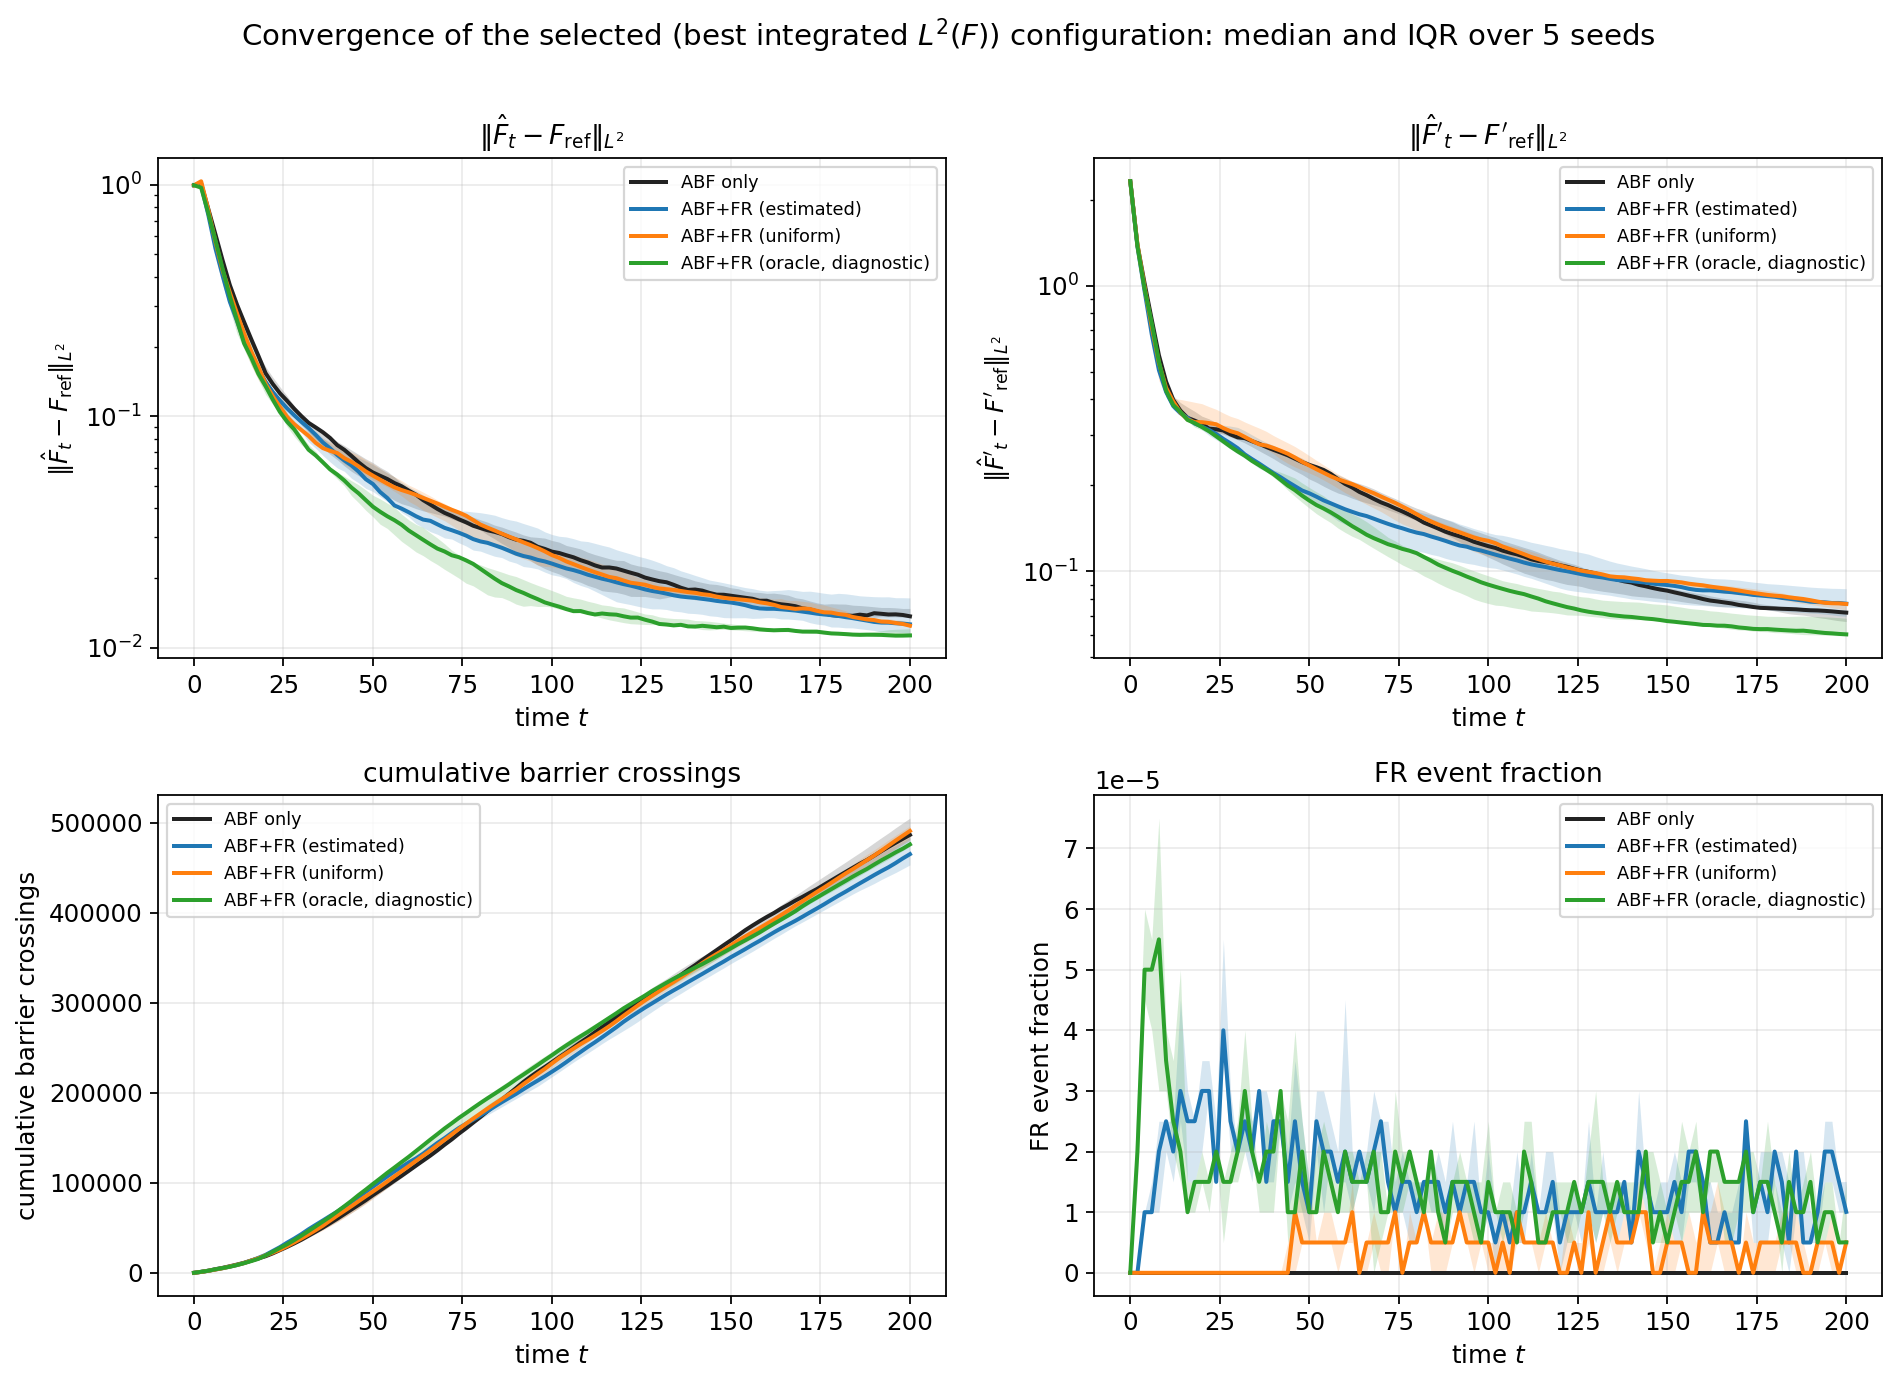
\includegraphics[width=0.95\textwidth]{fig02_convergence_curves.png}
  \caption{Convergence of the selected (integrated-$\Ltwo(F)$ rule)
    configuration for each method: median (line) and inter-quartile range
    (band) over \NSeeds{} seeds. The free-energy and mean-force errors
    (top, log scale) fall fastest for the oracle diagnostic and faster for the
    estimated/uniform FR than for ABF only in the early-to-middle phase;
    barrier crossings (bottom left) are essentially indistinguishable, and the
    FR event fraction (bottom right) is of order $10^{-5}$ throughout. The oracle
    curve is a diagnostic control (\cref{rem:oracle}).}
  \label{fig:convergence}
\end{figure}

\subsubsection{Final profiles and target-type ablation}
\Cref{fig:profiles} overlays the final mean-force, free-energy and
reaction-coordinate-marginal profiles. All practical methods recover
$\Fpref$ and $\Fref$ well; the visible differences between ABF only and
ABF+FR estimated at the final budget are small, consistent with the modest
final-error improvements. The $x$-marginal (panel c) is somewhat flatter under
FR, as intended, but marginal flatness is a diagnostic, not the goal.

\begin{figure}[t]
  \centering
  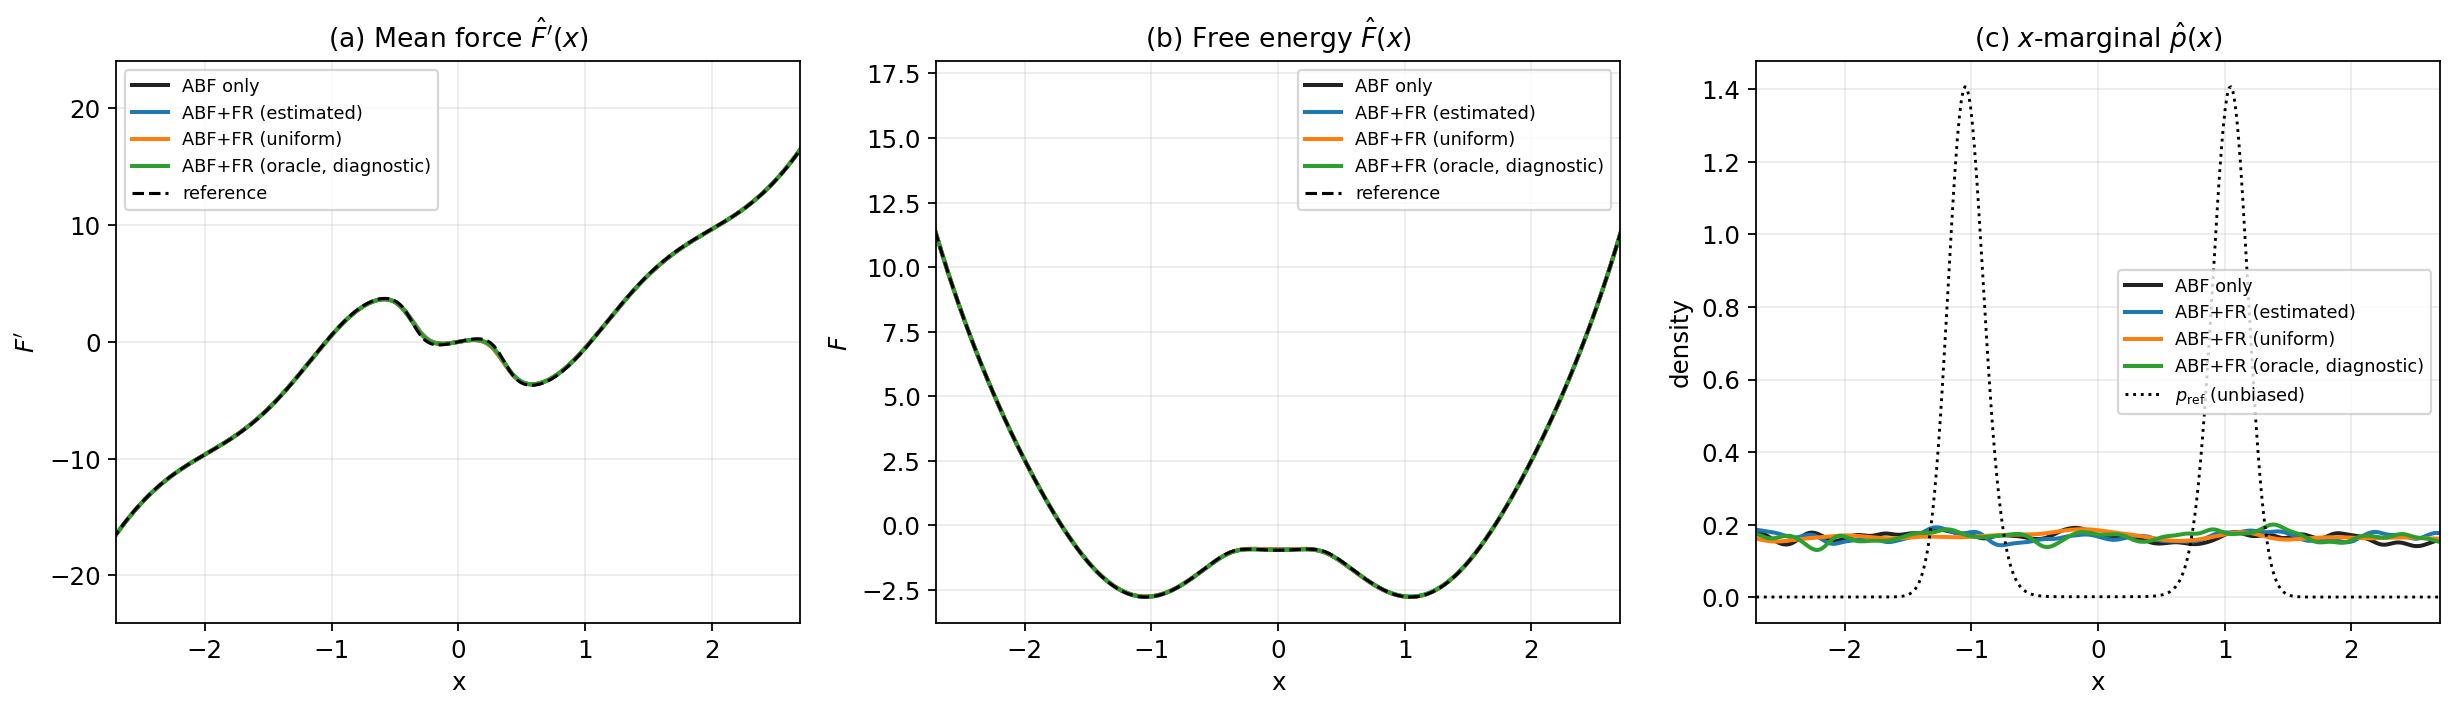
\includegraphics[width=0.97\textwidth]{fig03_final_profiles.png}
  \caption{Final profiles (mean over seeds) for the selected configurations.
    (a) Mean force $\Fphat(x)$ and (b) centred free energy $\Fhat(x)$ versus the
    reference (dashed); (c) reaction-coordinate marginal $\phat(x)$, with the
    unbiased $\pref$ (dotted). Practical methods recover the reference well; FR
    mildly flattens $\phat$.}
  \label{fig:profiles}
\end{figure}

\Cref{fig:ablation} shows the distribution, over the \NFRconfigs{}
configurations of each target type, of the seed-median errors. For the
\emph{integrated} error all three FR target types have medians below the
ABF-only baseline, but the spread is wide and some configurations are
\emph{worse} than ABF, so FR does not help unconditionally. For the \emph{final}
$\Ltwo(F)$ the estimated and uniform medians sit essentially on the ABF baseline,
and on the final \emph{mean-force} error they lie slightly \emph{above} it ---
only the oracle control is consistently below. Flattening the marginal with an
imperfect target buys early speed but not final mean-force accuracy.

\begin{figure}[t]
  \centering
  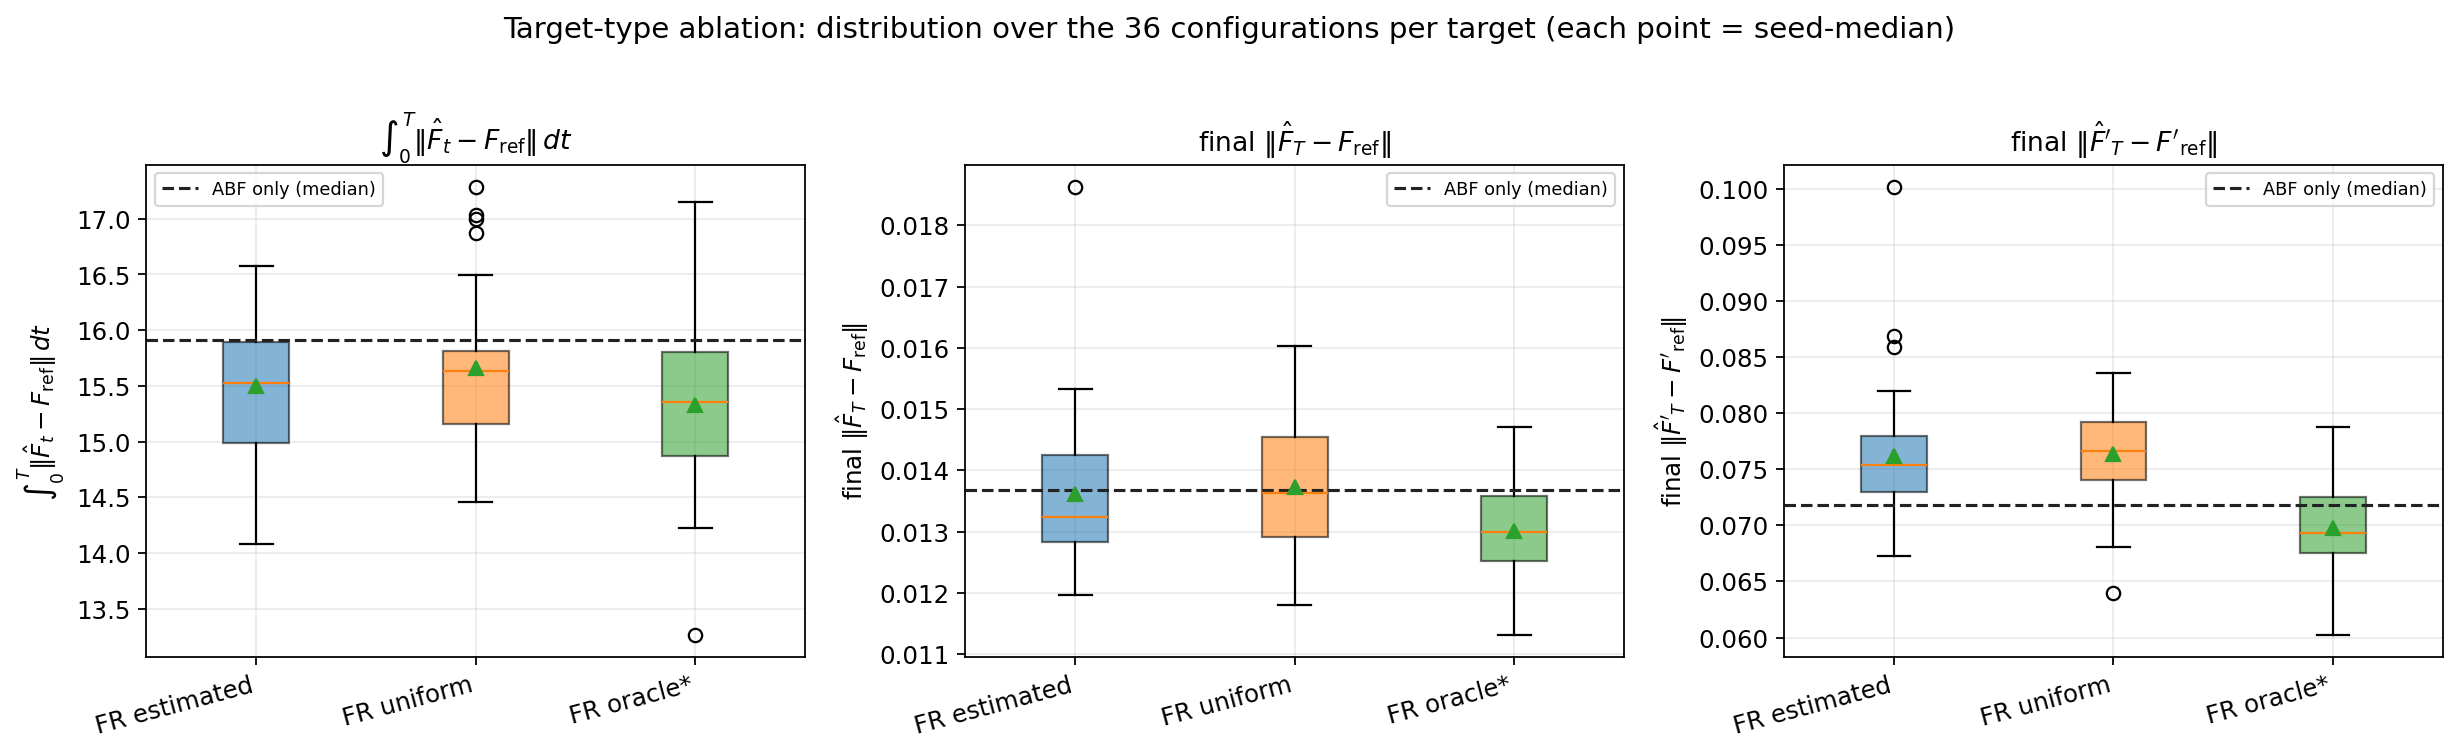
\includegraphics[width=0.97\textwidth]{fig04_target_ablation.png}
  \caption{Target-type ablation: each box is the distribution over the
    \NFRconfigs{} configurations of a target type (each point a seed-median);
    the dashed line is the ABF-only median. FR lowers the \emph{integrated}
    error (left) but the practical targets barely change the \emph{final}
    $\Ltwo(F)$ (middle) and slightly raise the final mean-force error (right).
    Only the oracle diagnostic improves all three.}
  \label{fig:ablation}
\end{figure}

\subsubsection{Two selection rules give different ``best'' hyperparameters}
\label{sec:selection}
Because integrated and final errors measure different things, they need not be
optimised by the same configuration. Selecting by \emph{integrated} $\Ltwo(F)$
(\cref{tab:main_integrated}) favours fast convergence and selects an aggressive
configuration for the estimated target ($\gamma=\EstIntGamma$, burn-in
$\EstIntBurnin$); selecting by \emph{final} $\Ltwo(F)$ (\cref{tab:main_final})
favours final-budget accuracy and selects a gentle, delayed configuration
($\gamma=\EstFinGamma$, burn-in $\EstFinBurnin$), which improves the final
free-energy error by $\EstFinFinalImpPct\%$ and beats ABF on $\EstFinProb\%$ of
matched seeds. This dependence on the selection rule is itself a finding.

\input{tables/best_configs_by_final_F.tex}

The \emph{uniform} target is competitive here (integrated reduction
$\UniIntegImpPct\%$): under a near-converged bias $\Bt\approx F$ the canonical
biased marginal is already close to uniform, so ``flatten $\phat$'' and ``match
the biased marginal'' nearly coincide. The \emph{oracle} diagnostic
(\cref{rem:oracle}) achieves the lowest errors of all (integrated reduction
$\OracIntegImpPct\%$), but it requires $\Fref$ and is unusable; the correct
reading is comparative: the estimated target captures $\EstIntegImpPct\%$ of the
reduction against the oracle's $\OracIntegImpPct\%$, so a substantial part of the
mechanism's potential is left unrealised by the online target estimate. In this
easy regime, then, the oracle--estimated gap localises the practical bottleneck
in the \emph{target estimation} --- a reading we revisit, and qualify, in
\cref{sec:synthesis}.

\subsection{Mechanism}
\label{sec:mechanism}
The mechanism is a feedback loop between coverage and the mean-force estimate.
ABF needs samples \emph{across} the reaction coordinate: by
\eqref{eq:meanforce}, $\Fpref(x)$ is a conditional average that can only be
estimated where particles visit $x$. Early in a run the bias is poor and the
ensemble is unbalanced --- \cref{fig:mechanism}(b) shows the initial occupancy
split ($\sim\!0.5$ in one basin) relaxing only gradually toward the balanced
$1/3$--$1/3$--$1/3$ split. FR compares $\phat_t$ with the target $q_t$ and
preferentially kills over-represented and clones under-represented particles
\eqref{eq:death}, raising the useful coverage of $x$ earlier than diffusion
alone would. Provided the birth--death does not corrupt $Y\mid X=x$
(\cref{prop:cond_invariance}), better coverage feeds back into a better
conditional mean-force estimate.

\begin{figure}[t]
  \centering
  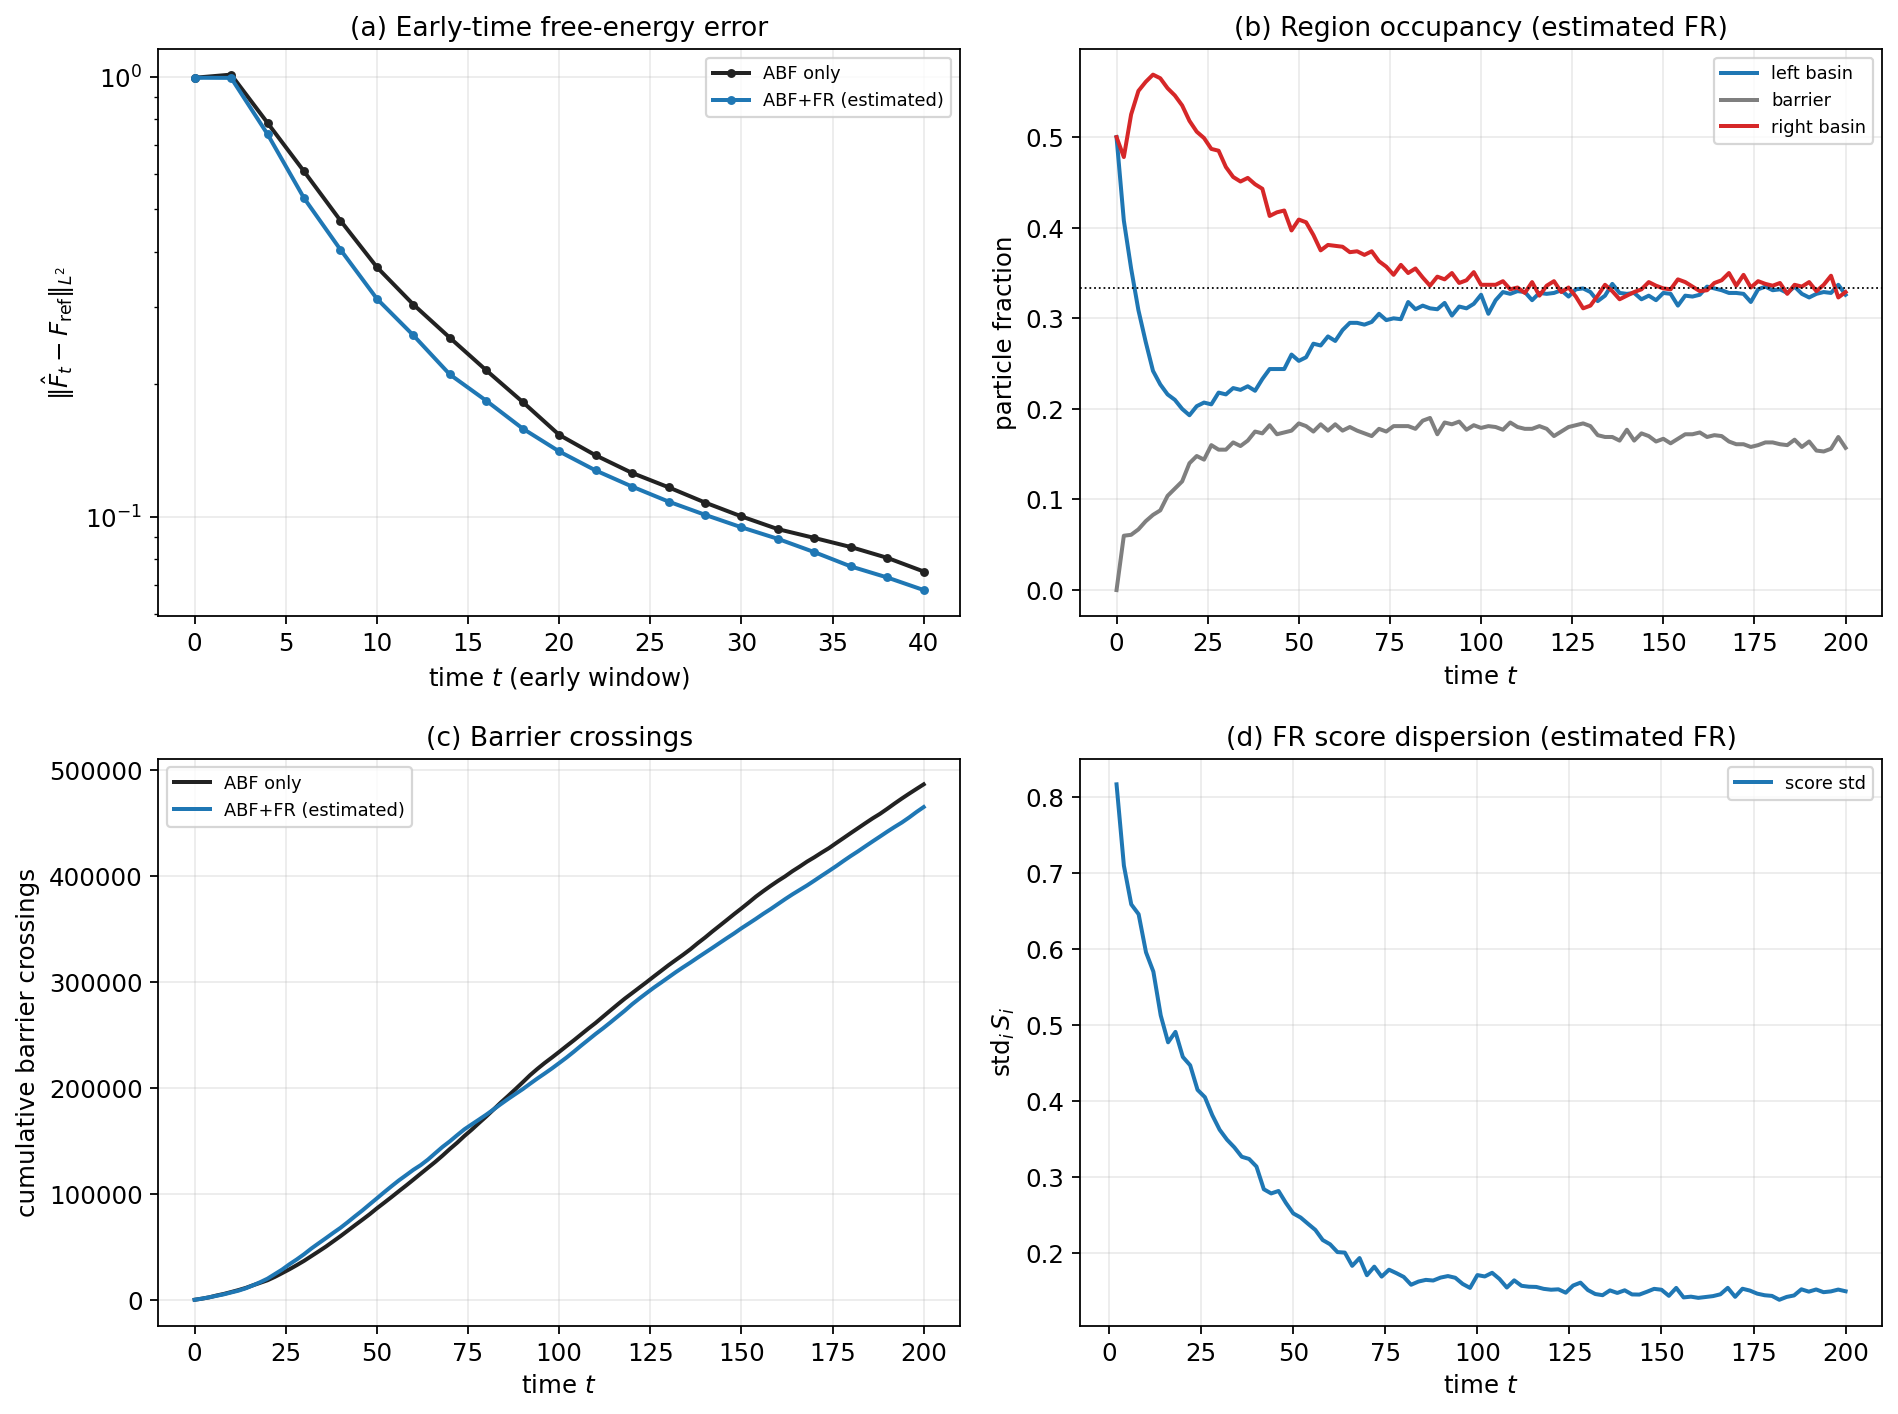
\includegraphics[width=0.95\textwidth]{fig05_mechanism.png}
  \caption{Mechanistic / early-time behaviour, estimated FR (best
    integrated-rule config) versus ABF only. (a) Early-time free-energy error
    (log scale): FR converges faster. (b) Region occupancy under FR relaxes
    from an unbalanced start toward the balanced $1/3$ split (dotted).
    (c) Cumulative barrier crossings are nearly identical --- the benefit here
    is redistribution, not a large increase in raw crossings. (d) FR score
    dispersion decays as $\phat_t\to q_t$.}
  \label{fig:mechanism}
\end{figure}

A notable feature of \cref{fig:mechanism}(c) is that FR does \emph{not} produce
many more barrier crossings than ABF; the benefit comes from \emph{reallocating}
existing replicas toward starved values of $x$ rather than from manufacturing
rare transitions. Consistent with this, the event fractions are of order
$10^{-5}$: in the successful regimes FR is a \emph{weak} correction.

\subsubsection{FR does not visibly corrupt \texorpdfstring{$Y\mid X=x$}{Y given X}}
\Cref{fig:conditional} compares the conditional fidelity of all methods at the
final time. The FR variants are \emph{not} worse than ABF only; near the barrier
($x\in\{-0.5,0,0.5\}$), where ABF-only under-samples, they are in fact slightly
\emph{better} on both the $\Ltwo$ and KL conditional metrics --- direct evidence
that the FR mechanism improves $x$-coverage without corrupting the orthogonal
sampling, the benign behaviour \cref{prop:cond_invariance} requires.

\begin{figure}[t]
  \centering
  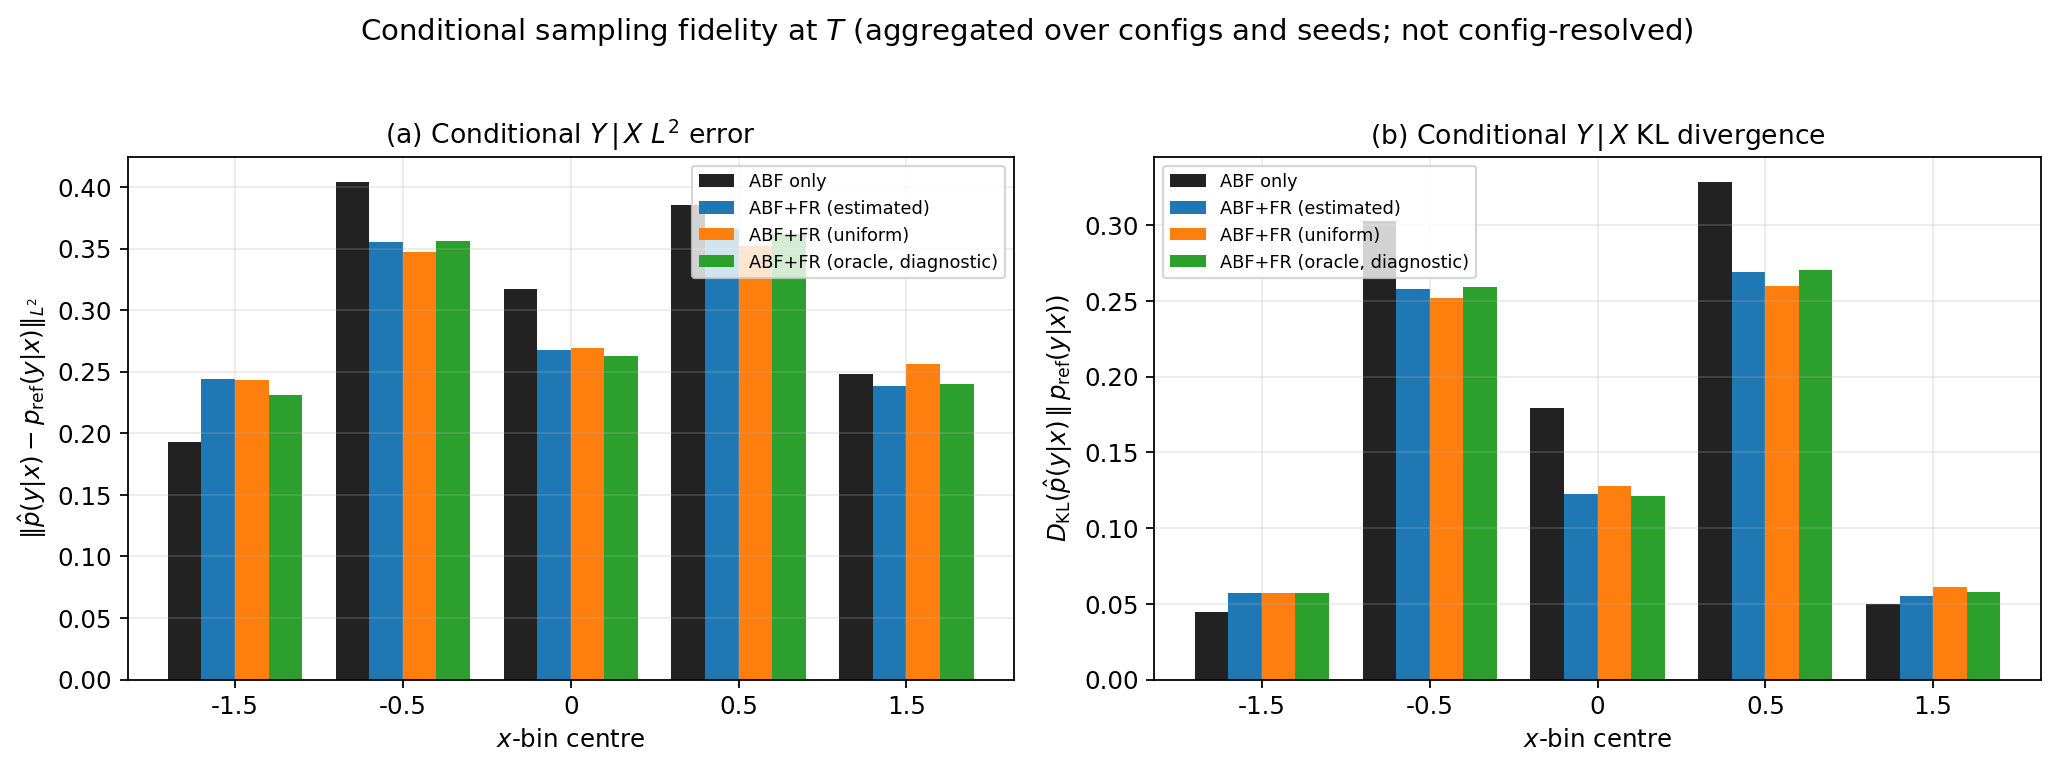
\includegraphics[width=0.95\textwidth]{fig06_conditional_y_given_x.png}
  \caption{Conditional $Y\mid X=x$ fidelity at $T$, by $x$-bin: (a) $\Ltwo$
    distance and (b) KL divergence of $\phat(y\mid x)$ to $\pref(y\mid x)$. FR
    does not inflate the conditional error; near the barrier it slightly reduces
    it. \emph{Limitation:} the conditional CSV identifies runs only by (method,
    target, seed) and is aggregated over configurations (\cref{rem:cond_limit}).}
  \label{fig:conditional}
\end{figure}

\begin{remark}[Conditional diagnostics are not configuration-resolved]
\label{rem:cond_limit}
The metastability conditional-diagnostics output records only (method, target
type, seed) per row, not the FR hyperparameters. It supports the \emph{aggregate}
statement that successful FR does not visibly corrupt $Y\mid X=x$, but cannot
isolate a specific ``good'' versus ``bad'' configuration's effect. The
entropic-bottleneck case (\cref{sec:case_eb}) closes this gap with an
\emph{analytic} conditional law.
\end{remark}

\subsubsection{What determines a good FR?}
\label{sec:q3}
\Cref{fig:hyper} (estimated target) shows the integrated error decreasing as
$\gamma$ grows --- a stronger correction converges faster, which is why the
integrated rule selects the aggressive $\gamma=\EstIntGamma$ --- but the same
setting does \emph{not} minimise the final error (\cref{sec:selection}): there is
an explicit speed-versus-accuracy trade-off in $\gamma$. The marginal bandwidth
$\eta$ is robust at intermediate values, and an early burn-in helps the
integrated error here because the largest imbalance is at early times. Across the
successful configurations the event fractions are tiny ($\sim10^{-5}$) and the
cap $f_{\max}$ never binds, so particle diversity is preserved.

\begin{figure}[t]
  \centering
  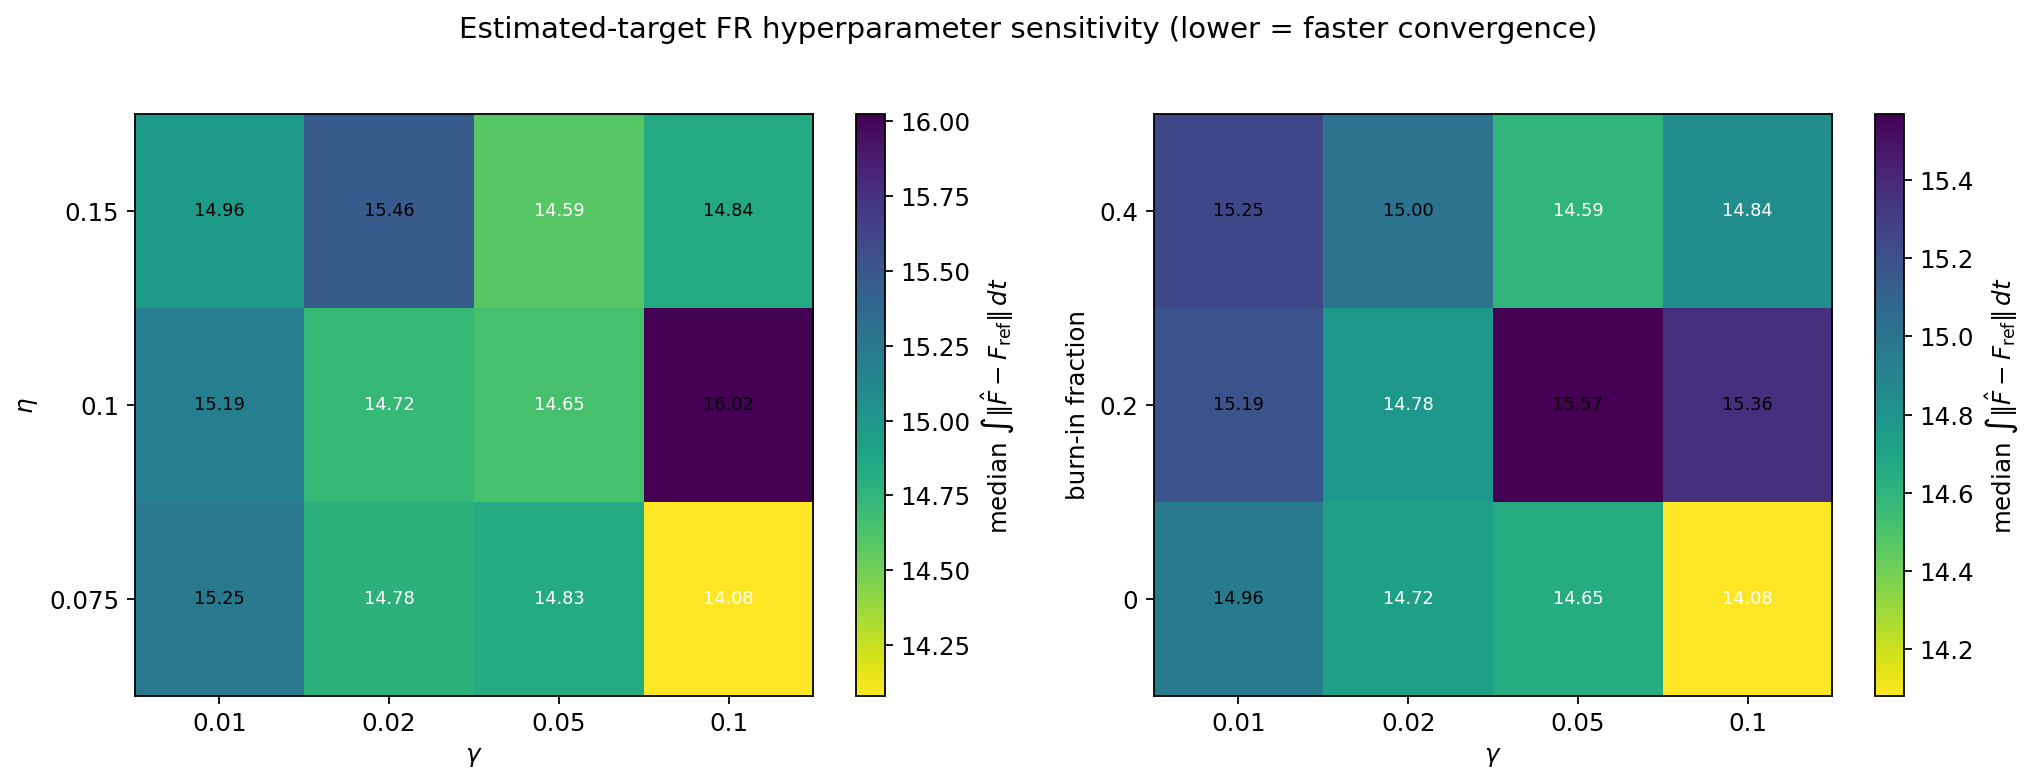
\includegraphics[width=0.95\textwidth]{fig07_hyperparameter_heatmaps.png}
  \caption{Estimated-target FR hyperparameter sensitivity: median integrated
    $\Ltwo(F)$ over the grid (lower = faster convergence). Left: $\gamma$ versus
    $\eta$; right: $\gamma$ versus burn-in fraction. The integrated error
    improves with larger $\gamma$ and earlier burn-in; intermediate $\eta$ is
    robust. These trends should not be extrapolated beyond this regime.}
  \label{fig:hyper}
\end{figure}

\subsection{Case finding}
\label{sec:q1}
On this easy metastability example the answer to Q1 is \emph{yes, but modestly,
and chiefly as a convergence accelerator}. Practical estimated-target FR improves
the integrated free-energy error by $\EstIntegImpPct\%$ with a smaller
final-budget gain; the improvement is real but not a rescue, and it is not
unconditional. Because plain ABF already converges well here, the room for FR to
help is small. The oracle control does best, which --- read \emph{within this
regime} --- points to target estimation as the practical bottleneck; we will see
in \cref{sec:case_eb,sec:case_wca} that this reading does not survive into the
starved regimes, where the oracle's advantage vanishes or reverses.

\section{Case II: an entropic bottleneck}
\label{sec:case_eb}

The second system tightens a transverse channel at the barrier top and, by
lowering the temperature, drives ABF into a genuinely sample-starved regime. It
also has a rare luxury: the conditional law $Y\mid X=x$ is \emph{analytic}, so we
can test \cref{prop:cond_invariance} directly rather than against a histogram.

\subsection{Model potential and reference}
The potential couples a symmetric double well in $x$ to a transverse harmonic
channel whose stiffness varies with $x$,
\begin{equation}
  V(x,y) = H\,(x^2-1)^2 + \tfrac12\,\omega(x)^2\,y^2,\qquad
  \omega(x) = \omega_{\mathrm{out}} +
    (\omega_{\mathrm{in}}-\omega_{\mathrm{out}})\,e^{-x^2/2s^2},
  \label{eq:eb_potential}
\end{equation}
with reaction coordinate $\xib(x,y)=x$. The stiffness $\omega(x)$ is large near
$x=0$ (a \emph{narrow channel at the barrier top}) and relaxes to
$\omega_{\mathrm{out}}$ in the wells. Because the $y$-integral is Gaussian, the
reference is analytic up to a constant:
\begin{equation}
  \Fref(x) = H\,(x^2-1)^2 + \beta^{-1}\log\omega(x) + C,\qquad
  \Fpref(x) = 4H\,x\,(x^2-1) + \beta^{-1}\,\omega'(x)/\omega(x),
  \label{eq:eb_ref}
\end{equation}
and, crucially, the conditional law is the exact Gaussian
\begin{equation}
  Y\mid X=x \;\sim\; \mathcal N\!\bigl(0,\;1/(\beta\,\omega(x)^2)\bigr).
  \label{eq:eb_conditional}
\end{equation}
The base regime is $\beta=8$, $H=2.5$, $\omega_{\mathrm{out}}=1$,
$\omega_{\mathrm{in}}=25$, $s=0.25$, with $N=256$ walkers, $\mathrm{d}t=10^{-3}$,
and $40\,000$ steps. The free energy is gauged at $x=0$ and all $\Ltwo$ errors are
RMS over the interior window $x\in[-1.5,1.5]$.

\paragraph{Why this is an entropic bottleneck --- and an honest caveat.}
Near $x=0$ the accessible $y$-width shrinks like $1/\omega(x)$: at the base
setting the transverse channel is $\omega_{\mathrm{in}}/\omega_{\mathrm{out}}=25$,
i.e.\ its standard deviation is $25\times$ narrower than in the wells,
contributing an \emph{entropic}
term $\beta^{-1}\log\omega(x)$ to the free energy. We are explicit, however, that
in this parameterisation the entropic barrier $\beta^{-1}\log\omega_{\mathrm{in}}
\approx 0.4$ is small next to the energetic barrier $4H\approx10$ (in $F$-units).
The bottleneck modulates the transverse width but is \emph{not} the dominant
contributor to reaction-coordinate starvation; that role belongs to the energetic
double well. This matters for reading the $\omega_{\mathrm{in}}$ sweep below.

\subsection{Methods and design}
The practical comparison is again \textbf{ABF only} versus \textbf{ABF+FR
estimated}~\eqref{eq:q_est}, on matched seeds (identical initial conditions and
Langevin noise per seed). The diagnostics \textbf{FR uniform}~\eqref{eq:q_unif}
and \textbf{FR oracle}~\eqref{eq:q_oracle} (built from the analytic $\Fref$, hence
not deployable, \cref{rem:oracle}) are also run. The FR hyperparameters are listed
in \cref{tab:eb_design}; an assertion guards every batched call so the reference
never reaches the estimated target.

\begin{table}[t]
\centering
\small
\caption{Entropic-bottleneck base regime and Fisher--Rao hyperparameters.}
\label{tab:eb_design}
\begin{tabular}{ll}
\toprule
Quantity & Value \\
\midrule
Inverse temperature $\beta$ & 8 \\
Barrier height $H$ & 2.5 \\
Channel stiffness $\omega_{\rm out},\omega_{\rm in}$ & 1, 25 \\
Channel width $s$ & 0.25 \\
Walkers $N$ & 256 \\
Time step $\Delta t$ & $10^{-3}$ \\
Steps per run & 40{,}000 \\
FR rate $\gamma$ & 15 \\
FR stride \texttt{fr\_every} & 10 \\
Score clip $S_{\max}$ & 3 \\
Event cap $f_{\max}$ & 0.08 \\
Target EMA rate & 0.005 \\
\bottomrule
\end{tabular}
\end{table}


\subsection{Results}
At the base regime the practical method reduces the median final free-energy
error from $\EBabfLtwoF$ (ABF) to $\EBfrLtwoF$ (ABF+FR estimated), a
$\EBgainStrong\%$ reduction, winning $\EBcoldWin$ of $20$ matched seeds
(\cref{fig:eb_convergence}). Two diagnostics are immediately revealing. The
\emph{uniform} target --- which carries no information about the free-energy
shape at all --- recovers almost the entire gain ($\EBuniGain\%$), while the
\emph{oracle} target (the \emph{analytic} $\Fref$) is \emph{worse than plain ABF}
($\EBoracleGain\%$). This is the opposite of the metastability ranking
(\cref{sec:q1}): here a target that over-commits to a fixed shape fights the ABF
bias instead of merely equalising coverage. The signature points to
\emph{balanced resampling / variance reduction across the reaction coordinate}, not
free-energy-shape steering, as the source of the gain.

\begin{figure}[t]
  \centering
  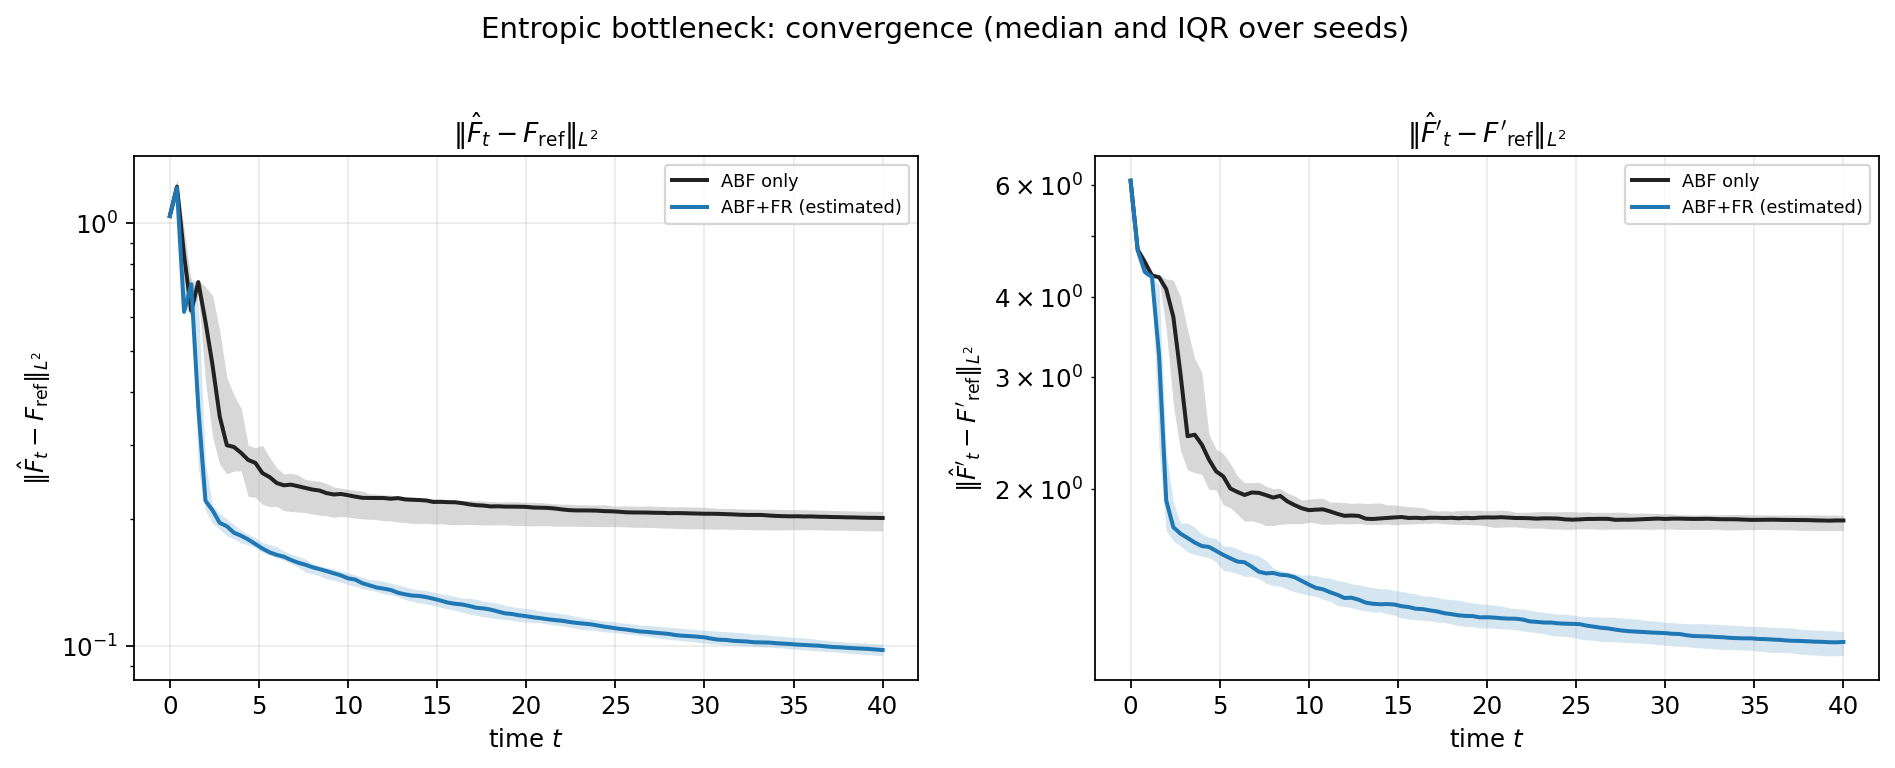
\includegraphics[width=0.92\textwidth]{fig_eb_01_convergence.png}
  \caption{Entropic bottleneck, convergence (median and inter-quartile range
    over seeds). ABF+FR estimated separates from ABF early and stays below it for
    the entire trajectory on both the free-energy (left) and mean-force (right)
    errors.}
  \label{fig:eb_convergence}
\end{figure}

\subsubsection{Temperature governs the gain, not the bottleneck width}
Varying the inverse temperature $\beta$ at fixed $\omega_{\mathrm{in}}=25$
(\cref{tab:eb_beta}) is the cleanest mechanistic signal in the study. FR
\emph{helps when sampling is hard and hurts when it is easy}: at high temperature
($\beta=2,4$) crossings are frequent, ABF already samples the whole coordinate
(its error is $\sim0.05$), and FR's birth--death merely injects resampling noise
--- it is mildly harmful and loses most seeds ($\EBwarmGainBetaFour\%$ at
$\beta=4$). At low temperature ($\beta=8,12$) crossings are rare, ABF is starved
on the far side of the barrier (error $0.2$--$0.4$), and FR's balanced resampling
substantially repairs the coverage, winning every seed. The cross-over sits
between $\beta=4$ and $\beta=8$.

\begin{table}[t]
\centering
\small
\caption{Temperature sweep at $\omega_{\rm in}=25$: the FR gain flips sign as ABF crosses from well-sampled (hot) to starved (cold).}
\label{tab:eb_beta}
\begin{tabular}{lrrrr}
\toprule
$\beta$ & ABF $\|F\!-\!F_{\rm ref}\|$ & FR $\|F\!-\!F_{\rm ref}\|$ & gain (\%) & win rate \\
\midrule
2 & 0.055 & 0.060 & -8.8 & 0.30 \\
4 & 0.049 & 0.062 & -26.1 & 0.00 \\
8 & 0.201 & 0.098 & +51.3 & 1.00 \\
12 & 0.416 & 0.281 & +32.3 & 1.00 \\
\bottomrule
\end{tabular}
\end{table}


By contrast, sweeping the bottleneck width $\omega_{\mathrm{in}}$ at fixed
$\beta=8$ (\cref{fig:eb_omega}) leaves the gain essentially \emph{flat} at
$\sim50\%$. This is the honest consequence of the caveat above: the ABF baseline
error is nearly independent of $\omega_{\mathrm{in}}$ because the
$\omega$-independent energetic barrier dominates the sampling difficulty. The
gain is large and reliable across $\omega_{\mathrm{in}}$, but it is governed by
metastability (temperature), not by the bottleneck width. We do not claim a
bottleneck-strength scaling the data do not show.

\begin{figure}[t]
  \centering
  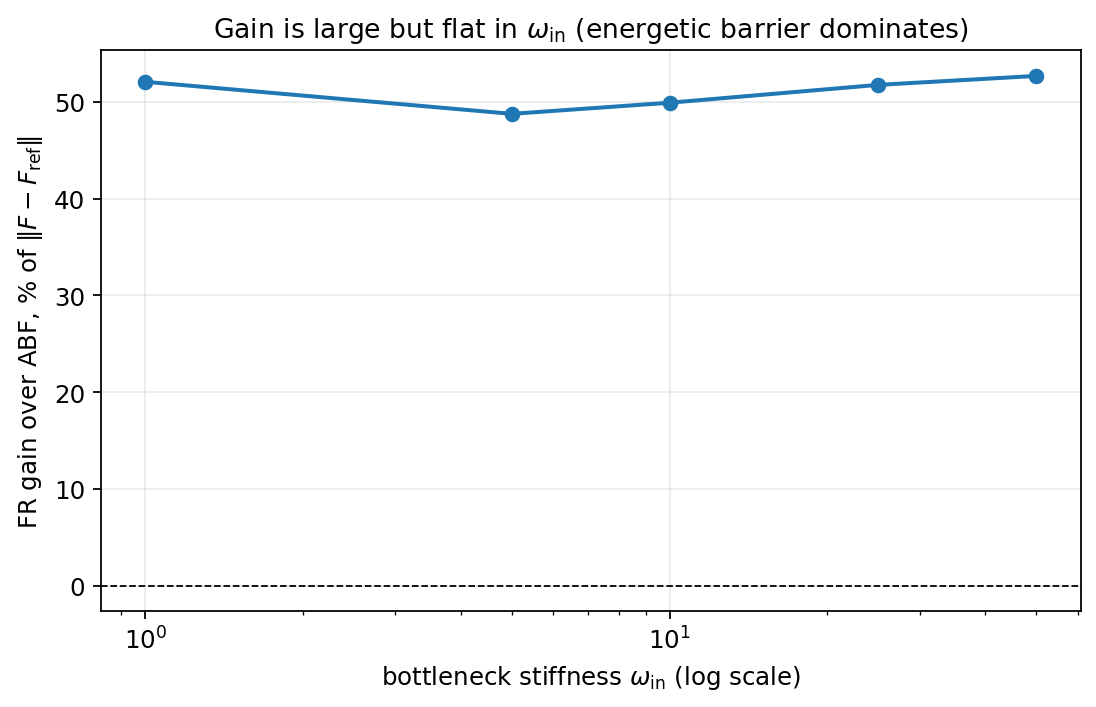
\includegraphics[width=0.92\textwidth]{fig_eb_02_omega.png}
  \caption{Bottleneck-width sweep $\omega_{\mathrm{in}}$ at $\beta=8$. The FR gain
    is large ($\sim50\%$) and $100\%$ reliable at every width, but it does
    \emph{not} grow with the bottleneck strength: the ABF baseline error is flat
    because the energetic barrier $4H\approx10$ dominates the sub-unit entropic
    barrier $\beta^{-1}\log\omega_{\mathrm{in}}$.}
  \label{fig:eb_omega}
\end{figure}

\subsubsection{A wide safe regime for the FR rate}
Sweeping the birth--death rate $\gamma$ at the base regime
(\cref{fig:eb_gamma}), the gain increases \emph{monotonically} up to
$\gamma=50$ ($+\EBgammaMaxGain\%$); we did not reach a failure boundary within the
swept range. The windowed ancestor effective sample size falls steadily from
$\EBessHi$ to $\EBessLo$ as lineage diversity collapses, yet the free-energy error
keeps improving. This differs from the WCA dimer (\cref{sec:case_wca}), where
aggressive birth--death eventually degrades the estimator; the likely reason is
the very short conditional-relaxation time of the analytic $y$-channel here, so a
cloned walker re-equilibrates its orthogonal coordinate almost immediately. FR is
unusually robust in this model.

\begin{figure}[t]
  \centering
  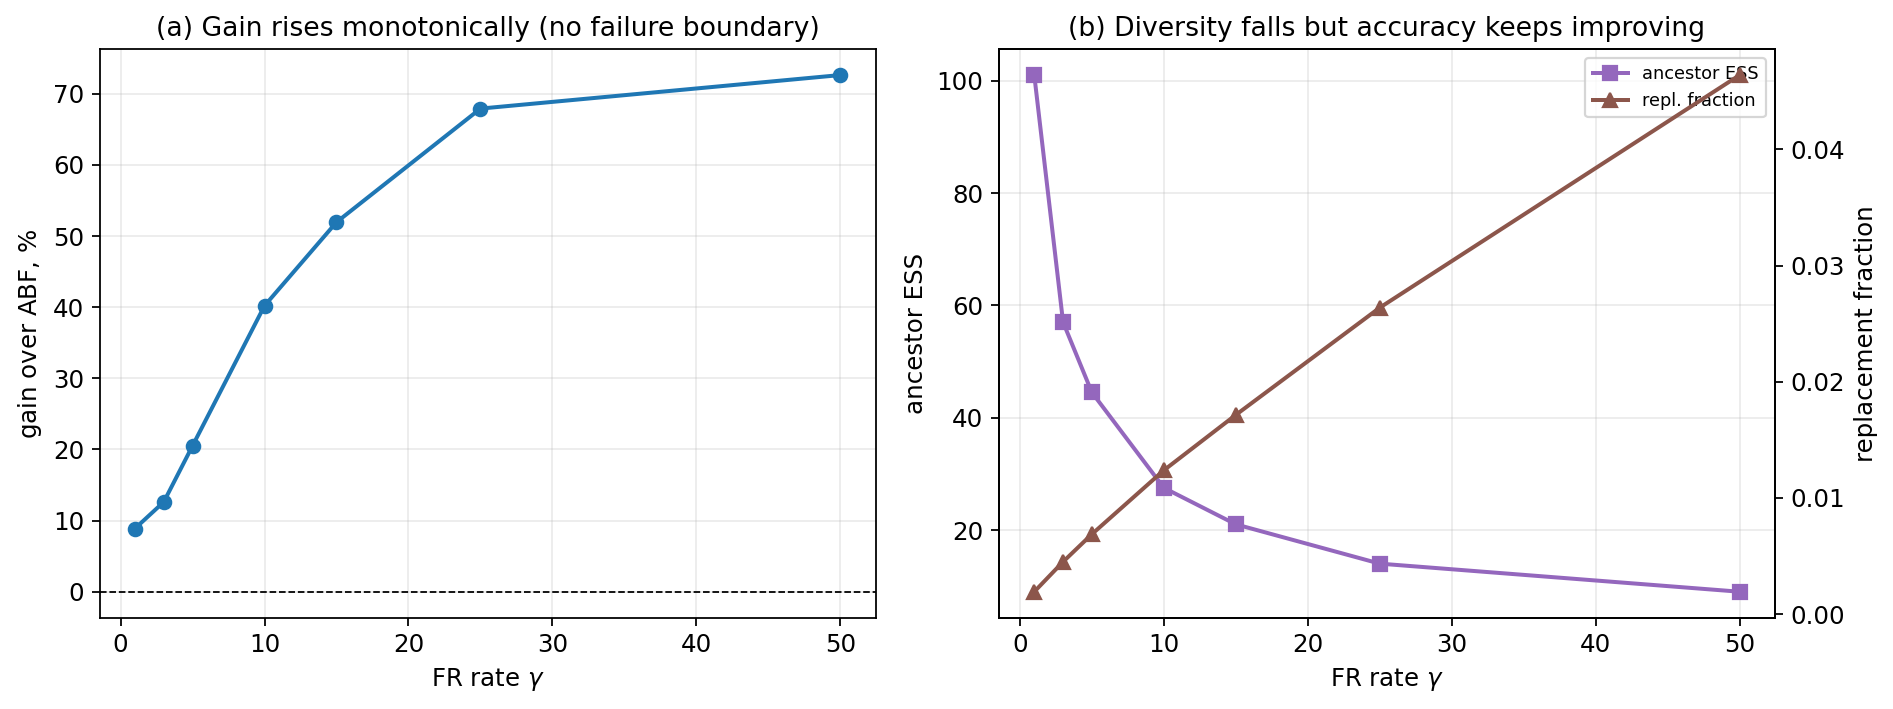
\includegraphics[width=0.92\textwidth]{fig_eb_03_gamma.png}
  \caption{FR-rate sweep $\gamma\in\{1,\dots,50\}$ at the base regime. Left: gain
    over ABF increases monotonically (no failure boundary in range). Right:
    windowed ancestor ESS collapses ($\EBessHi\to\EBessLo$) and the replacement
    fraction rises, yet accuracy keeps improving.}
  \label{fig:eb_gamma}
\end{figure}

\subsection{Mechanism: conditional fidelity from an analytic law}
Because $Y\mid X=x\sim\mathcal N(0,1/(\beta\omega(x)^2))$ is \emph{analytic}
\eqref{eq:eb_conditional}, we can test \cref{prop:cond_invariance} directly rather
than against a noisy histogram --- the gap that \cref{rem:cond_limit} left open in
the metastability case. \Cref{fig:eb_conditional} compares the empirical
$\widehat{\mathrm{Var}}(Y\mid X\in I_j)$ to $1/(\beta\omega(x_j)^2)$ at five
$x$-bins. \textbf{FR preserves the conditional law}: at every bin the FR variance
tracks the analytic value as well as ABF does, across nearly three orders of
magnitude (from $\sim2\times10^{-4}$ at the bottleneck $x=0$ to $\sim0.12$ in the
wells), including the extremely narrow channel at $x=0$. The residual errors are
dominated by bin-count noise, not by any systematic FR distortion. The
free-energy improvement is therefore achieved \emph{without} corrupting the
orthogonal degrees of freedom --- exactly the benign behaviour
\cref{prop:cond_invariance} requires, now confirmed against an exact
conditional.

\begin{figure}[t]
  \centering
  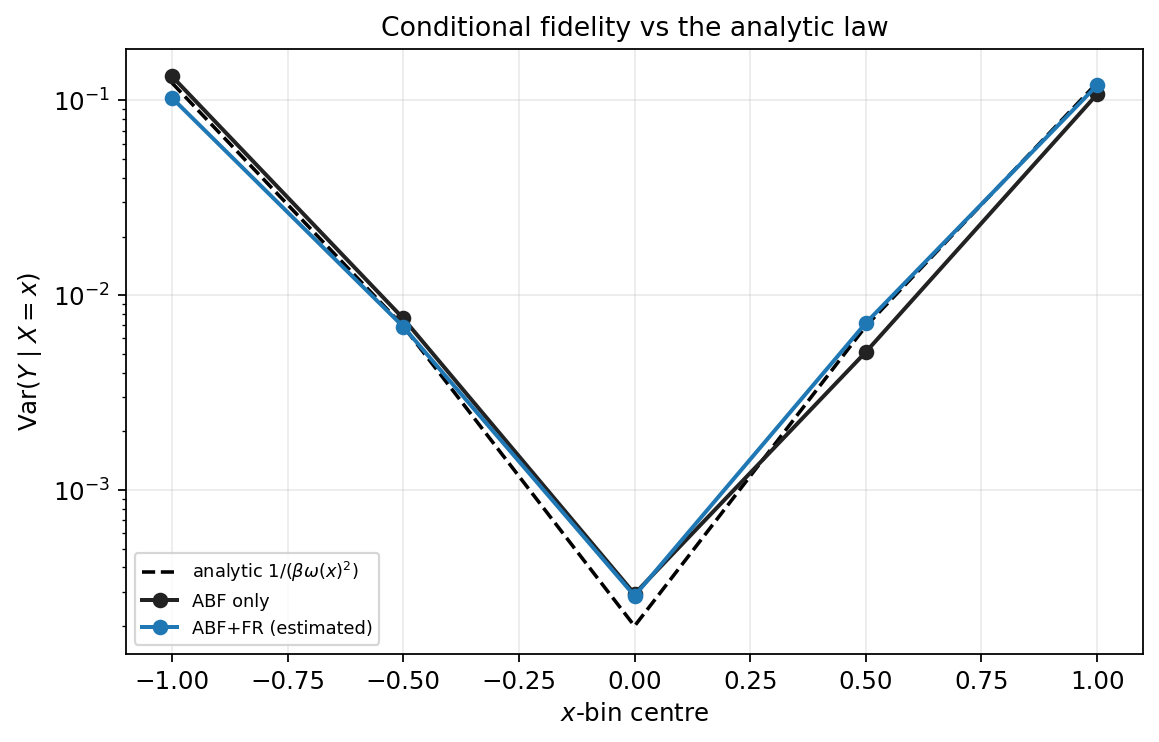
\includegraphics[width=0.92\textwidth]{fig_eb_04_conditional.png}
  \caption{Conditional fidelity against the \emph{analytic} law
    $\mathrm{Var}(Y\mid X=x)=1/(\beta\omega(x)^2)$. Empirical FR and ABF variances
    both track the analytic curve across three orders of magnitude; FR is not
    worse than ABF at any bin, including the narrow channel at $x=0$.}
  \label{fig:eb_conditional}
\end{figure}

\subsection{Case finding}
The entropic bottleneck is a controlled bridge between the easy metastability case
and the hard WCA dimer. Estimated-target FR robustly and substantially reduces the
free-energy error in the cold, sample-starved regime ($\sim\EBgainStrong\%$,
$\EBcoldWin/20$ seeds), but the gain is governed by \emph{temperature} (FR helps
when ABF is starved, mildly hurts when it is not), not by the bottleneck width.
The mechanism is balanced resampling / variance reduction, not shape steering:
the uniform target nearly matches the estimated one and the oracle target is
\emph{worse} than ABF --- the reverse of the metastability ranking. The safe FR
regime is wide (no failure boundary up to $\gamma=50$), and, thanks to the
analytic conditional, we confirm directly that successful FR does not corrupt
$Y\mid X=x$.

\section{Case III: a condensed-phase WCA dimer}
\label{sec:case_wca}

The third system is many-body and is where ABF is most starved: a dimer that must
push a dense solvent aside to change its bond length. It tests whether the
two-dimensional findings survive in a setting with thousands of degrees of freedom
and a nonlinear collective variable.

\subsection{Model and reference}
A dimer of two tagged particles sits in a periodic two-dimensional bath of
$n_{\mathrm{dim}}^2-2$ Weeks--Chandler--Andersen (WCA) solvent particles
($n_{\mathrm{dim}}=10$, lattice spacing $a$, box $L=n_{\mathrm{dim}}\,a$). All
particles interact through the purely repulsive WCA
potential~\citep{WeeksChandlerAndersen1971} (Lennard--Jones cut and shifted at its
minimum $r_0=2^{1/6}\sigma$). The two dimer particles additionally feel a symmetric
double-well bond $V_{\mathrm{dim}}(r)=h\,(1-((r-r_0-w)/w)^2)^2$ with barrier
height $h=2$ and width $w=2$. The reaction coordinate is the scaled bond length
\begin{equation}
  z(q) = \frac{|q_1-q_2|-r_0}{2w},
  \label{eq:wca_cv}
\end{equation}
a nonlinear collective variable of the full configuration $q\in\R^{2n}$
(\cref{rem:manybody}): $z\approx0$ is the \emph{compact} state, $z\approx1$ the
\emph{stretched} state, and $z\in[0.25,0.75]$ the \emph{transition} region. The
free-energy barrier near $z=0.5$ is partly entropic / crowding-driven, since the
dimer must displace solvent to cross it. Dynamics are overdamped Langevin at
$\beta=1$, $\mathrm{d}t=0.002$, with the minimum-image convention; the default
system is $a=1.5$, $\sigma=\epsilon=1$. The local mean force along $z$ is the
constrained projection of the physical forces plus the geometric $2w/(\beta r)$
term (\cref{rem:manybody}). The reference $F(z)$ is computed once per system $a$ by
constrained-MD thermodynamic integration~\citep{Carter1989,DenOtterBriels1998}
and used for evaluation only; errors are taken on the interior window
$z\in[-0.1,1.1]$ with the additive constant aligned.

\subsection{Methods and design}
As before the practical comparison is \textbf{ABF only} versus \textbf{ABF+FR
estimated}~\eqref{eq:q_est}, with \textbf{FR uniform} and \textbf{FR oracle}
diagnostics; here the oracle target is built from the TI reference and is
explicitly \emph{not} deployable (\cref{rem:oracle}). A no-leakage assertion
ensures only the oracle method ever receives the reference, and a clone copies the
\emph{entire} WCA configuration --- not just $z$ --- so cloned solvent
arrangements travel with the bond length. Replica lineage is tracked to report the
ancestor effective sample size $\mathrm{ESS}=1/\sum_a w_a^2$. The tuned FR
configuration is given in \cref{tab:wca_design}; the rate is named
\texttt{fr\_rate} and the onset \texttt{fr\_start\_steps} (\cref{sec:fr_notation}).

\begin{table}[t]
\centering
\small
\caption{WCA dimer base system and tuned Fisher--Rao hyperparameters.}
\label{tab:wca_design}
\begin{tabular}{ll}
\toprule
Quantity & Value \\
\midrule
Inverse temperature $\beta$ & 1 \\
Time step $\Delta t$ & 0.002 \\
Steps per run & 250{,}000 \\
Replicas $N$ & 1024 \\
Lattice spacing $a$ & 1.5 \\
Dimer barrier $h$, width $w$ & 2, 2 \\
FR rate \texttt{fr\_rate} & 0.10 \\
FR onset \texttt{fr\_start\_steps} & 20{,}000 \\
FR stride \texttt{fr\_every} & 5 \\
Score clip $S_{\max}$ & 2.0 \\
Event cap $f_{\max}$ & 0.02 \\
Target EMA rate & 0.005 \\
\bottomrule
\end{tabular}
\end{table}


\subsection{Results}
The main comparison (\cref{tab:wca_main}; 10 seeds, $N=1024$, $250\,000$ steps)
shows the practical method \textbf{reliably beating ABF}: the tuned FR cuts the
median final $\Ltwo(F)$ from $\WCAabfLtwoF$ to $\WCAtunedLtwoF$
(\,$+\WCAtunedGainPct\%$\,), winning all $\WCAtunedWin/10$ matched seeds. As in the
entropic-bottleneck case, the uniform target ($+\WCAuniGainPct\%$) and the oracle
target ($+\WCAoracleGainPct\%$) are \emph{essentially as good as} the estimated
target --- the online estimated target already extracts nearly all the available
benefit, and there is no headroom to the oracle. We are explicit that the headline
gain is in the \emph{free energy}: the mean-force error $\Ltwo(F')$ improves only
modestly ($\approx22\%$), so we do not claim a large mean-force improvement.

\begin{table}[t]
\centering
\small
\caption{WCA main comparison (250k steps, $N=1024$, $a=1.5$). The headline gain is in the free energy; the mean-force gain is modest.}
\label{tab:wca_main}
\begin{tabular}{lrrrrr}
\toprule
Method & $\|F\!-\!F_{\rm ref}\|$ & $\|F'\!-\!F'_{\rm ref}\|$ & gain (\%) & wins & anc. ESS \\
\midrule
ABF only & 0.0835 & 0.3220 & -- & -- & -- \\
FR estimated (tuned) & 0.0361 & 0.2513 & +55.0 & 10/10 & 86 \\
FR uniform & 0.0372 & 0.2525 & +54.6 & 10/10 & 90 \\
FR oracle$^{*}$ & 0.0387 & 0.2475 & +52.7 & 10/10 & 100 \\
FR estimated (strong) & 0.0329 & 0.2590 & +58.9 & 10/10 & 45 \\
FR estimated (aggressive) & 0.0935 & 0.3883 & -13.1 & 1/10 & 22 \\
\bottomrule
\end{tabular}
\par\smallskip\footnotesize $^{*}$\,The oracle target uses the thermodynamic-integration reference $F_{\rm ref}$; it is a diagnostic control, \emph{not} a deployable method. Medians over $10$ seeds.
\end{table}


\begin{figure}[t]
  \centering
  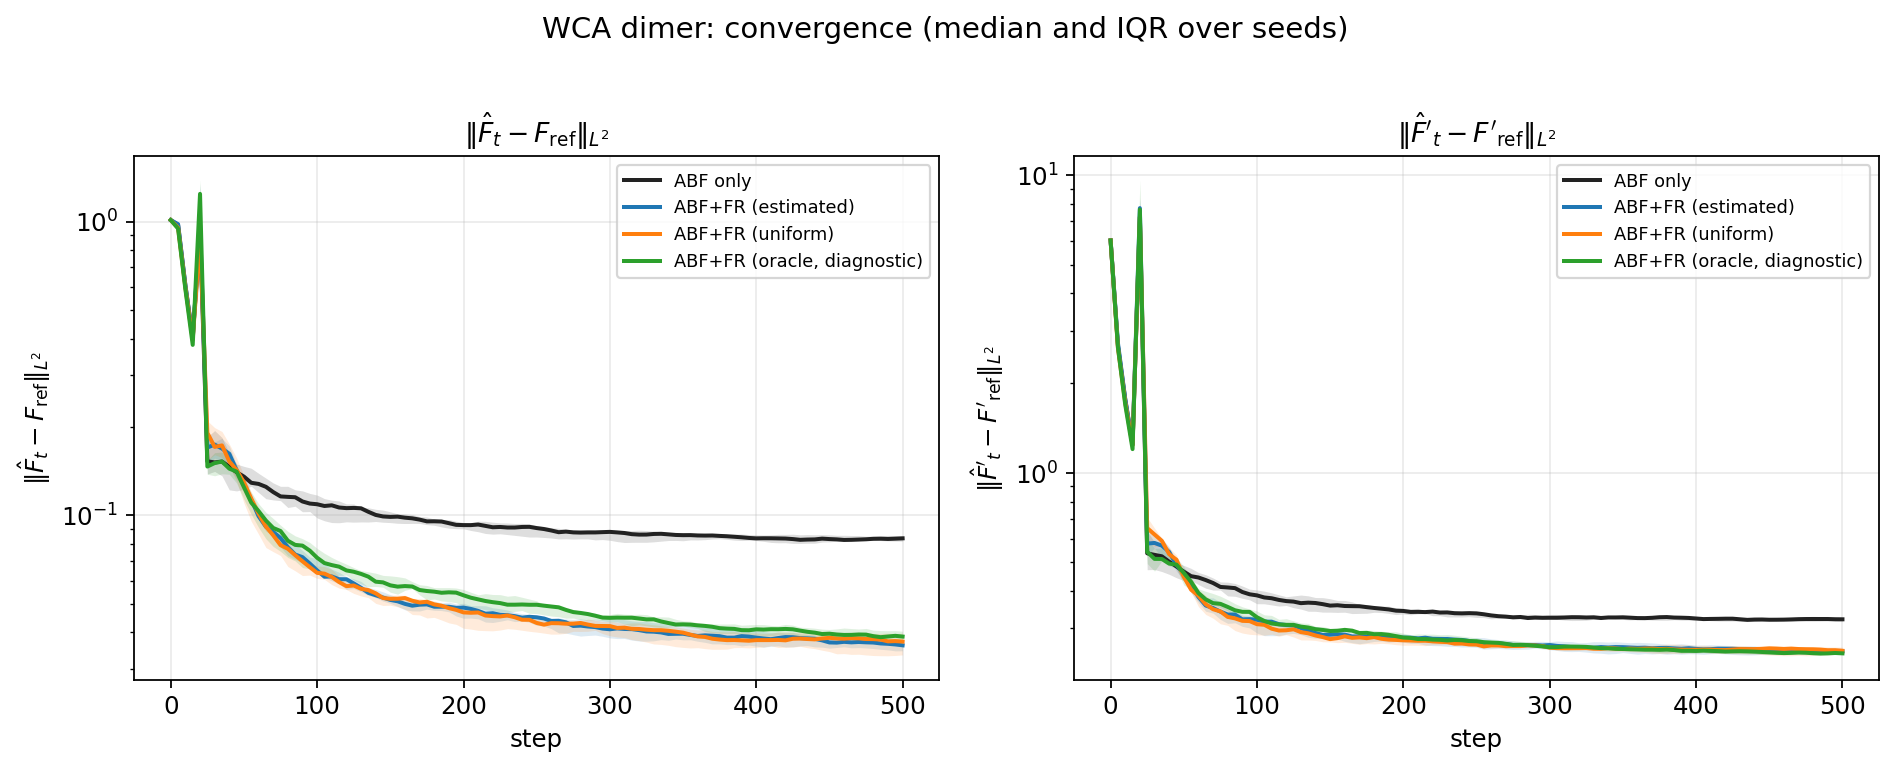
\includegraphics[width=0.92\textwidth]{fig_wca_01_convergence.png}
  \caption{WCA dimer, convergence (median and inter-quartile range over seeds).
    ABF and FR are identical until FR activates; from then on FR is consistently
    below ABF on $\Ltwo(F)$ for the rest of the run. The cumulative replacement
    count (right) confirms the birth--death is active but bounded.}
  \label{fig:wca_convergence}
\end{figure}

\begin{figure}[t]
  \centering
  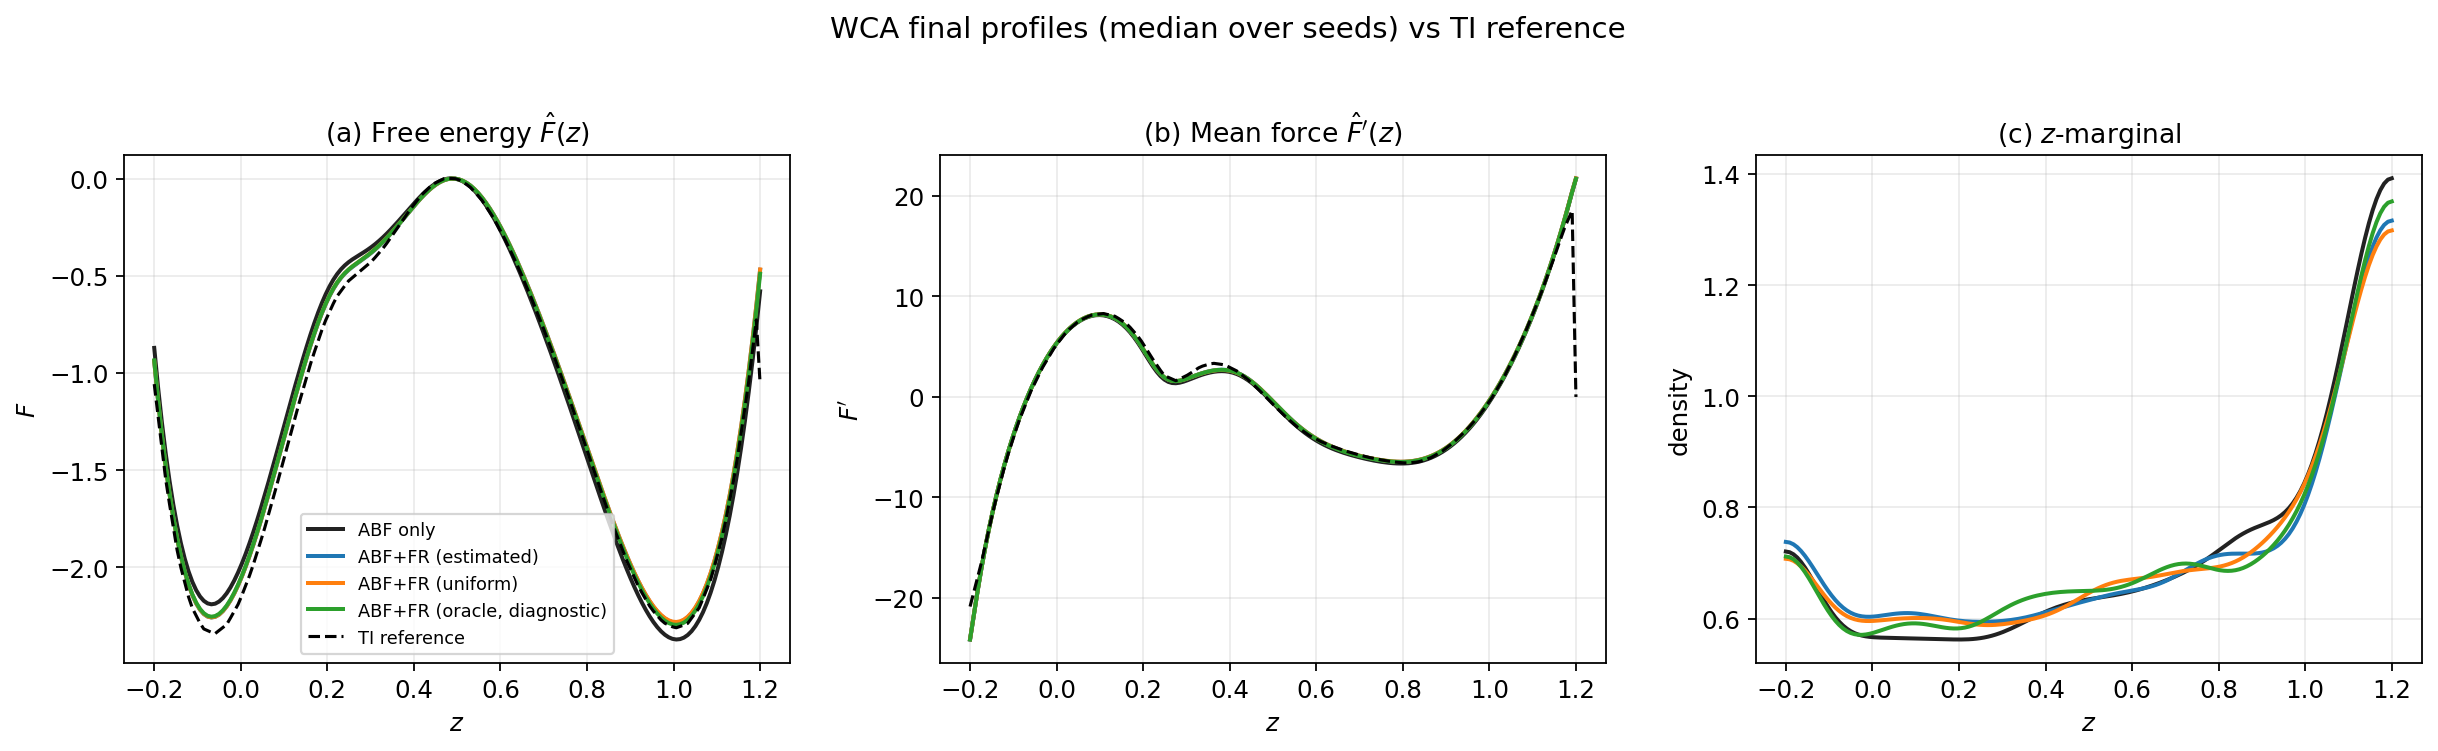
\includegraphics[width=0.92\textwidth]{fig_wca_02_profiles.png}
  \caption{Final profiles (median over seeds) versus the TI reference (dashed):
    (a) free energy $\Fhat(z)$, (b) mean force $\Fphat(z)$, (c) reaction-coordinate
    marginal. FR recovers the reference free energy more accurately than ABF,
    chiefly in and around the transition region.}
  \label{fig:wca_profiles}
\end{figure}

\subsection{Mechanism: resampling-driven variance reduction}
The diagnostics support the same mechanism as the entropic bottleneck rather than
a coverage-reshaping one. Final reaction-coordinate region fractions and the
fraction of effective ABF samples in the transition window are nearly identical
across ABF, FR estimated, FR uniform and FR oracle: FR does \emph{not} converge to
a different stationary $z$-distribution. Instead the gain appears immediately after
FR activates and is sustained for the rest of the run. \Cref{fig:wca_mechanism}
shows the interpretation: birth--death acts as a \emph{variance-reduction
resampler for the ABF estimator}. Replicas stuck in over-represented
configurations are replaced by whole-configuration clones of under-represented
ones, raising the number of effectively-independent force samples per $z$-bin even
when the marginal looks unchanged. Because the \emph{entire} WCA configuration is
copied (\cref{rem:manybody}), clones inject decorrelated solvent arrangements,
accelerating convergence of $\Fhat$ without requiring a different stationary
coverage --- consistent with $\text{uniform}\approx\text{estimated}\approx
\text{oracle}$.

\begin{figure}[t]
  \centering
  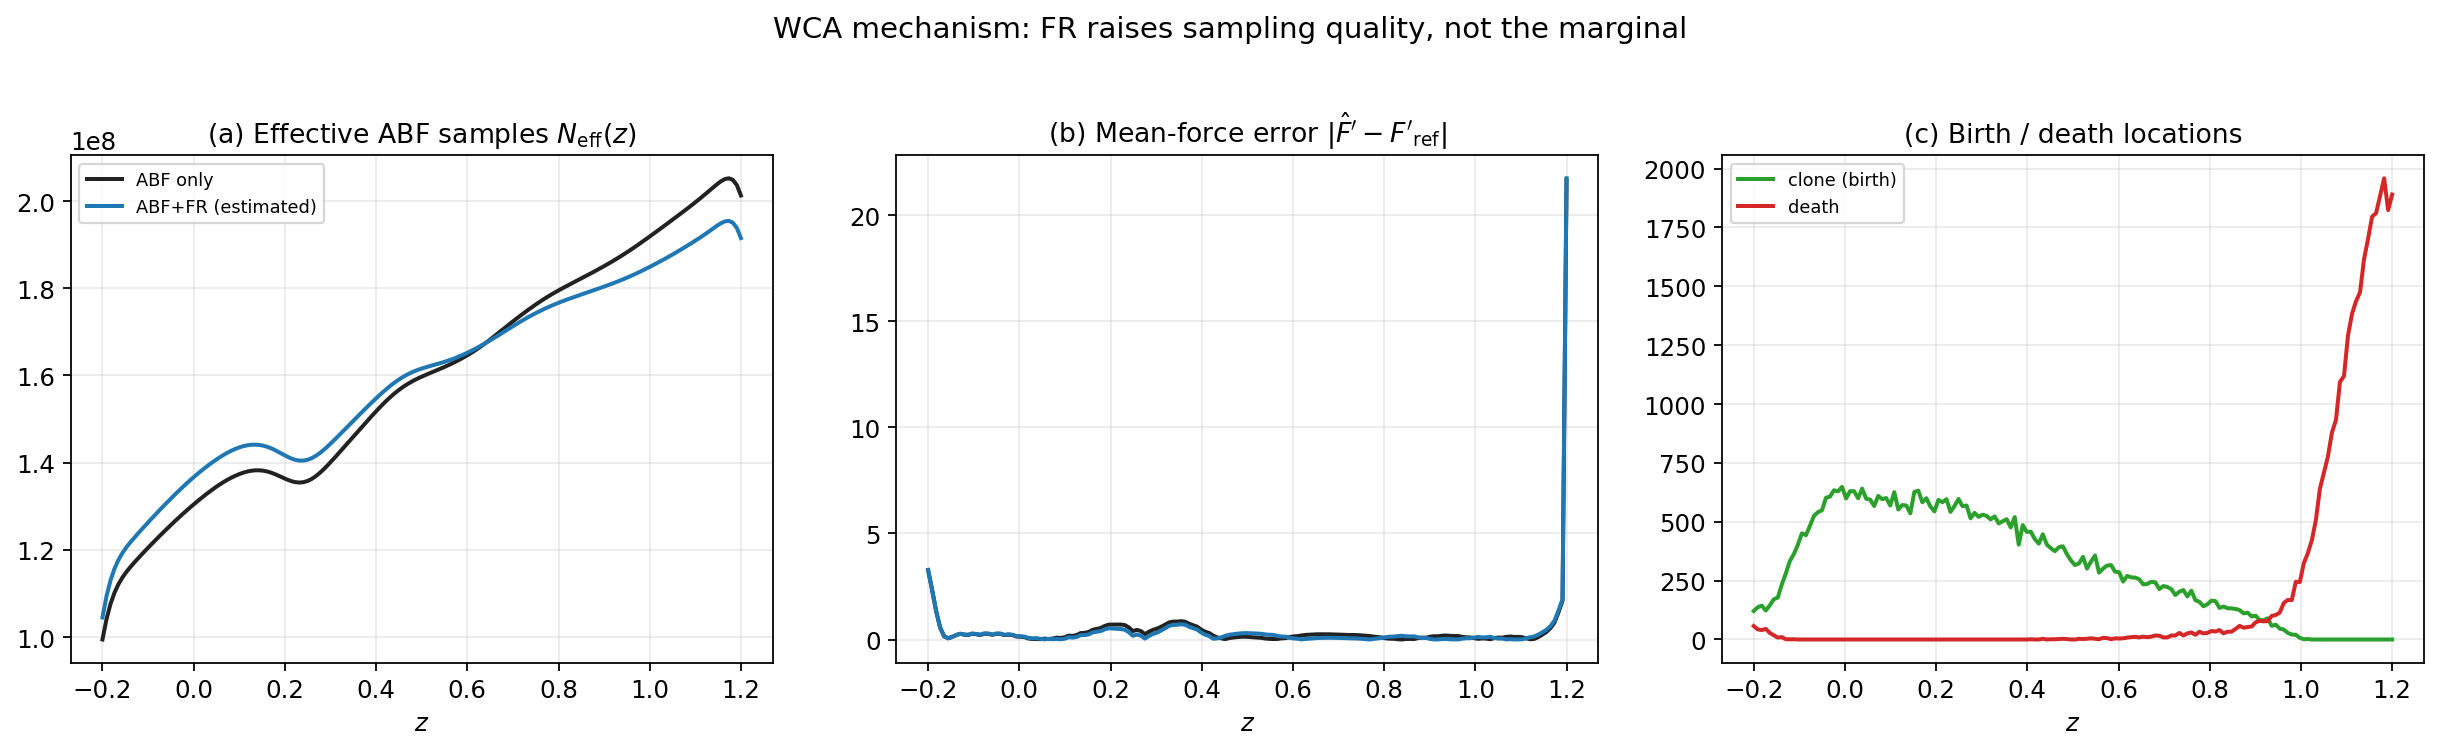
\includegraphics[width=0.92\textwidth]{fig_wca_04_mechanism.png}
  \caption{Mechanism. (a) Effective ABF sample count $N_{\mathrm{eff}}(z)$ is
    raised by FR in the transition window; (b) per-bin mean-force error is reduced
    there; (c) birth (clone) and death locations concentrate around the
    over/under-sampled regions; FR reshapes the \emph{sampling quality}, not the
    stationary marginal.}
  \label{fig:wca_mechanism}
\end{figure}

\subsection{Failure boundary}
Unlike the entropic bottleneck, the WCA dimer exhibits a clear failure boundary in
the FR rate (\cref{fig:wca_failure}). The rate ladder (a shorter $150$k-step,
$4$-seed stage) maps a clean safe regime: too gentle
(\texttt{fr\_rate}$\le0.05$) gives a small gain ($+19$--$29\%$); the sweet spot
(\texttt{fr\_rate}$\approx0.1$--$0.2$) gives the maximal $+58$--$64\%$ with healthy
ancestor ESS; the gain then \emph{erodes} sharply
(\texttt{fr\_rate}$=0.5$ falls to $+12\%$ with the error already climbing back
toward the ABF baseline) and finally \emph{reverses} for
\texttt{fr\_rate}$\ge1$, where the median final $\Ltwo(F)$ is worse than ABF
($-38\%$ at rate $1$, $-68\%$ at rate $2$) and no seed wins, as the ancestor ESS
collapses from $\sim\!337$ to $\sim\!20$. The reversal arrives even earlier under a
longer budget: the production aggressive configuration (\texttt{fr\_rate}$=0.5$ at
$250$k steps, $10$ seeds) is already net-harmful ($\WCAaggrGainPct\%$, winning only
$1/10$ seeds, ancestor ESS $\sim\!22$), because the extra steps give diversity loss
more time to dominate. Over-aggressive birth--death destroys the replica diversity
the mean-force estimator depends on, so the estimator degrades faster than coverage
improves. This is the predicted failure mode; the analytic $y$-channel of the
entropic bottleneck masks it (\cref{sec:case_eb}) because cloned walkers
re-equilibrate instantly, whereas a dense solvent does not.

\begin{figure}[t]
  \centering
  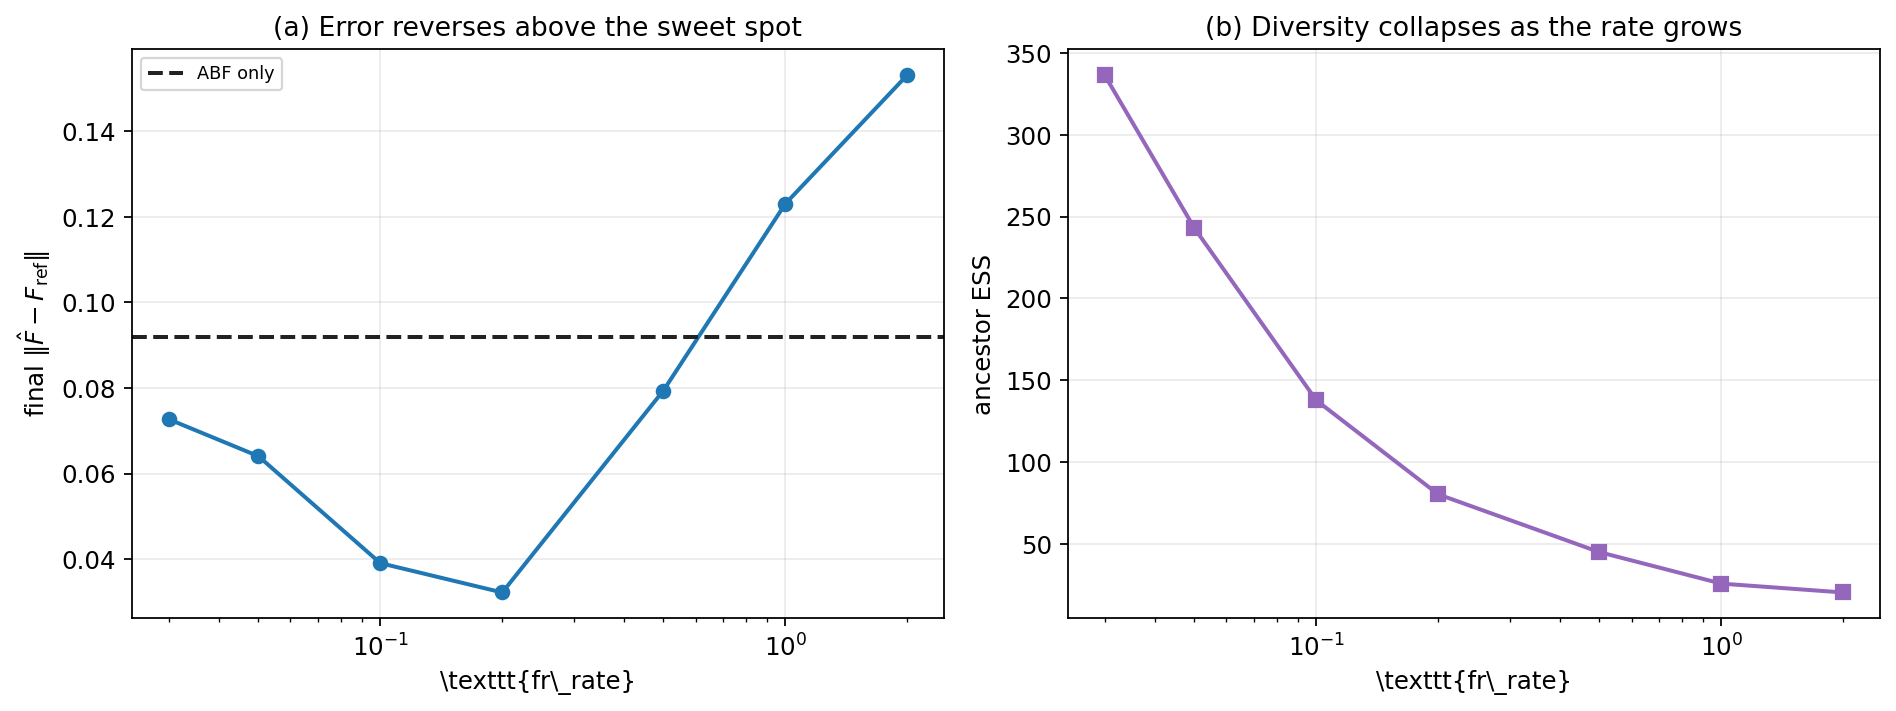
\includegraphics[width=0.92\textwidth]{fig_wca_05_failure.png}
  \caption{FR-rate ladder ($150$k steps, $4$ seeds). Final $\Ltwo(F)$ (left) is
    minimised in the $0.1$--$0.2$ sweet spot, climbs back toward the ABF baseline
    (dashed) by \texttt{fr\_rate}$=0.5$, and rises above it for
    \texttt{fr\_rate}$\ge1$; ancestor ESS (right) collapses as the rate grows,
    pinpointing diversity loss as the failure mechanism.}
  \label{fig:wca_failure}
\end{figure}

\subsection{Difficulty dependence}
Varying one difficulty axis at a time (\cref{fig:wca_difficulty}) shows the gain
is robust and, importantly, \emph{grows with difficulty}. With \emph{budget}, FR
wins at every $n_{\mathrm{steps}}$ and the relative advantage grows rather than
washes out ($+\WCAbudgetLoGain\%$ at $50$k to $+\WCAbudgetHiGain\%$ at $400$k):
ABF's error plateaus around $0.08$ after $\sim150$k while FR keeps descending, so
FR is not merely an early-time accelerator that ABF later catches. With
\emph{replica count}, the gain is roughly flat ($+51$--$59\%$ from $N=256$ to
$2048$) --- FR helps even at $N=256$. With \emph{solvent crowding}, the densest
bath ($a=1.35$) makes the entropic barrier severe and ABF $\sim4\times$ worse in
absolute error; FR still wins $5/5$ and delivers by far the largest absolute error
reduction ($\WCAdenseAbfErr\to\WCAdenseFrErr$). In the units a practitioner cares
about --- absolute free-energy error removed --- the crowded regime is where FR
helps most.

\begin{figure}[t]
  \centering
  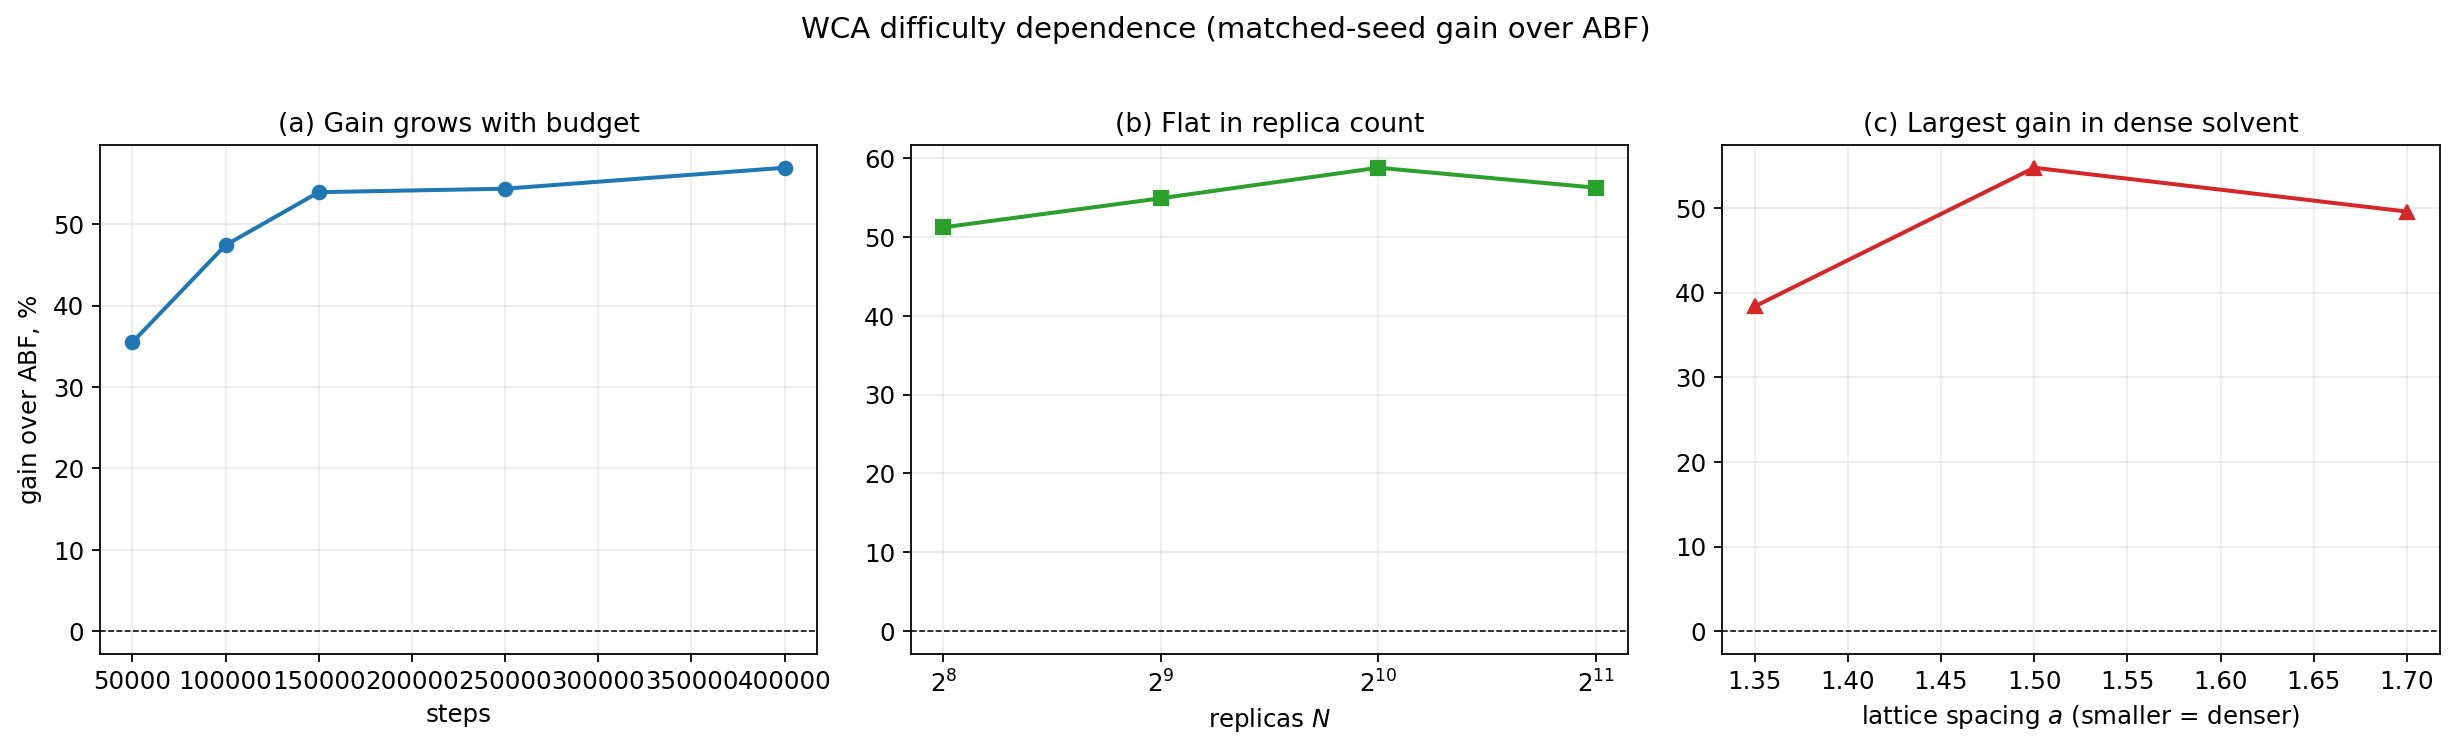
\includegraphics[width=0.95\textwidth]{fig_wca_06_difficulty.png}
  \caption{Difficulty dependence (matched-seed gain over ABF). (a) Budget: the
    relative gain grows with $n_{\mathrm{steps}}$ as ABF plateaus and FR keeps
    improving. (b) Replica count: gain is roughly flat. (c) Solvent crowding:
    smaller $a$ (denser) yields the largest absolute error reduction. FR wins
    $5/5$ seeds in every cell.}
  \label{fig:wca_difficulty}
\end{figure}

\subsection{Case finding}
On the condensed-phase WCA dimer, ABF+FR with an online estimated target reliably
and substantially improves free-energy accuracy: $+\WCAtunedGainPct\%$ in median
final $\Ltwo(F)$ at the tuned operating point, winning $\WCAtunedWin/10$ seeds,
with the gain concentrated in the free energy (not the mean force). The mechanism
is balanced-resampling variance reduction after warm-up; the precise target shape
matters little ($\text{uniform}\approx\text{estimated}\approx\text{oracle}$, and
the estimated target already reaches the oracle's accuracy). The method has a clear
safe regime, \texttt{fr\_rate}$\approx0.1$--$0.2$, and a real failure boundary:
too-aggressive birth--death reverses the benefit as diversity collapses. The
advantage \emph{grows with simulation budget}, is insensitive to replica count, and
is largest in the densest, hardest solvent --- exactly the starved regime the
variance-reduction mechanism predicts.

\section{Cross-case synthesis}
\label{sec:synthesis}

The three cases were chosen to span a single axis: \emph{how sample-starved ABF
is}. Read together they tell a more coherent story than any one of them does
alone, and they resolve an apparent contradiction in how the FR \emph{target}
behaves.

\subsection{A starvation spectrum}
Order the cases by how badly plain ABF is starved of reaction-coordinate samples.
At the easy end is the metastability model (\cref{sec:case_meta}), where ABF
already converges well; in the middle is the entropic bottleneck
(\cref{sec:case_eb}), whose difficulty we can dial with temperature; at the hard
end is the condensed-phase WCA dimer (\cref{sec:case_wca}), where the dimer must
displace a dense solvent to cross the barrier. \Cref{tab:synthesis} lays the
headline numbers side by side.

\begin{table}[t]
\centering
\small
\caption{Cross-case synthesis: the estimated-target FR gain grows with how sample-starved ABF is, while the value of the target \emph{shape} (oracle vs.\ estimated) shrinks. Metastability gain is on the integrated error; the others on final $\|F-F_{\rm ref}\|$.}
\label{tab:synthesis}
\begin{tabular}{lllll}
\toprule
Case & Regime & FR gain (\%) & wins & target effect \\
\midrule
Metastability & ABF strong & +11.5 (int.) & -- & oracle best \\
Entropic bottleneck (hot, $\beta{=}4$) & ABF easy & -26.1 & 0/10 & n/a \\
Entropic bottleneck (cold, $\beta{=}8$) & ABF starved & +51.3 & 20/20 & oracle worse \\
WCA dimer & ABF starved & +55.0 & 10/10 & oracle $\approx$ est. \\
\bottomrule
\end{tabular}
\end{table}


\subsection{The gain grows with starvation}
The practical, estimated-target FR gain tracks the starvation axis almost
monotonically. Where ABF is a strong baseline the gain is small and not
unconditional --- $+\EstIntegImpPct\%$ on the integrated error in the
metastability case, with a marginal final-budget gain --- and where ABF is even
less stressed (the hot entropic bottleneck, $\beta\le4$) FR is mildly
\emph{harmful} ($\EBwarmGainBetaFour\%$ at $\beta=4$), because its birth--death
injects resampling noise into an estimator that was not starved to begin with.
Where ABF is starved the gain is large and reliable: $+\EBgainStrong\%$ in the
cold bottleneck ($\EBcoldWin/20$ seeds) and $+\WCAtunedGainPct\%$ on the WCA dimer
($\WCAtunedWin/10$ seeds), the relative gain growing further with simulation
budget and the largest \emph{absolute} error removed in the densest solvent. The entropic-bottleneck temperature sweep is the cleanest evidence
because it moves along the axis \emph{within a single system}: the same model, the
same code, the gain flipping sign from $\beta=4$ to $\beta=8$ as ABF crosses from
well-sampled to starved.

\subsection{Why the target shape matters less than it first seemed}
The cases appear to disagree about the FR \emph{target}. In the easy metastability
case the oracle target is best and the estimated--oracle gap reads as a
``target-quality bottleneck'' (\cref{sec:q1}). In the WCA dimer the oracle is no
better than the estimated or uniform target, and in the entropic bottleneck the
oracle is actually \emph{worse than plain ABF}. These are not contradictory once
the mechanism is separated from the target.

The \emph{dominant} effect of FR is balanced-resampling variance reduction:
killing over-represented and cloning under-represented whole configurations raises
the number of effectively independent force samples per reaction-coordinate bin,
which is exactly what a starved ABF estimator lacks. This effect needs only a
roughly correct \emph{direction} of imbalance, not an accurate free-energy shape
--- which is why the uniform target nearly matches the estimated one in both
starved cases. Target-shape steering is a \emph{secondary} effect that becomes
visible only when the variance-reduction headroom is already exhausted, i.e.\ when
ABF is well-sampled: there the residual error is limited by the target
\emph{direction}, so the oracle (which knows the exact direction) helps. When ABF
is starved the residual error is variance-limited, the exact shape is irrelevant,
and a target that over-commits to a fixed shape --- the oracle, anchored to a
$\Fref$ that the running bias has not yet matched --- can actively fight the bias
and lose to a neutral uniform target. The metastability ``target-quality
bottleneck'' is therefore a regime-specific reading, not a general law; we are
careful not to carry it into the starved regimes.

\subsection{A single failure mechanism: diversity collapse}
Both the safe regimes and the one observed failure are explained by the same
quantity --- ancestor diversity. Aggressive birth--death erodes the effective
number of independent lineages; the gain survives only while the orthogonal
degrees of freedom re-equilibrate fast enough to re-decorrelate the clones. The
WCA dimer reaches the failure boundary (\texttt{fr\_rate}$\ge1$ reverses the
benefit in the rate ladder, and even \texttt{fr\_rate}$=0.5$ becomes harmful at
production budget, ancestor ESS $\to\!20$--$22$) because its dense solvent
re-equilibrates slowly:
clones stay correlated and the estimator degrades. The entropic bottleneck does
\emph{not} reach a failure boundary even at $\gamma=50$ (ESS $\to\EBessLo$) because
its analytic $y$-channel re-equilibrates almost instantly, so even heavy cloning
does not starve the estimator within the budget. Same mechanism, different
orthogonal relaxation times --- which is why a safe FR rate must be calibrated to
how quickly the orthogonal coordinates of \emph{the system at hand} mix.

\section{Discussion, limitations, and future directions}
\label{sec:discussion}

\subsection{What the three cases establish (Q4)}
The original single-case study could only ask whether FR was ``icing on the
cake'' (a mild accelerator when ABF already works) or ``snow in the winter'' (a
rescue when ABF alone struggles), and explicitly deferred the question to harder
regimes. The two new cases \emph{are} those harder regimes --- lower temperature,
fewer particles, and a condensed phase --- and the answer is now \emph{both}: FR
is icing for easy ABF (metastability; hot bottleneck) and snow for starved ABF
(cold bottleneck; dense WCA dimer), with the transition governed by how
sample-starved ABF is (\cref{sec:synthesis}).

\subsection{Limitations}
We remain deliberately conservative about scope.
\begin{enumerate}
  \item \textbf{The reaction coordinates are low-dimensional.} All three systems
        use a one-dimensional reaction coordinate (a Cartesian component in the
        2D cases, a scalar bond length in WCA). Multi-dimensional or strongly
        curved collective variables, where the geometric mean-force term and the
        conditional sampling are far harder, are untested.
  \item \textbf{The oracle target is not a method.} In every case the oracle uses
        the reference free energy, the unknown being computed, and is reported
        only as a diagnostic control (\cref{rem:oracle}). Its behaviour is read
        only comparatively; notably, it is \emph{not} uniformly best --- it is
        worse than ABF in the entropic bottleneck --- which is itself part of the
        synthesis, not a deployable result.
  \item \textbf{Production estimators are validated surrogates.} The 2D GPU
        backend uses a binned-smoothed mean-force/marginal estimator and a
        vectorised fixed-$N$ birth--death; the WCA backend uses a constrained
        projection with the geometric term. These pass their validation suites
        and agree with the kernel/TI references to within tolerance, but are not
        bit-identical to the original kernel notebook implementation.
  \item \textbf{Metastability conditional diagnostics are not
        configuration-resolved} (\cref{rem:cond_limit}). The entropic-bottleneck
        case closes this gap with an analytic conditional law, but only for that
        model; the WCA conditional fidelity is argued structurally
        (\cref{rem:manybody}) rather than measured per configuration.
  \item \textbf{The entropic barrier is sub-dominant in Case II.} As stated in
        \cref{sec:case_eb}, the bottleneck modulates the transverse width but the
        energetic double well dominates the difficulty; the $\omega_{\mathrm{in}}$
        sweep is honestly flat, and we do not claim a bottleneck-strength scaling.
\end{enumerate}

\subsection{Failure modes}
The analysis points to a single unifying failure mechanism, diversity collapse,
plus target misspecification (\cref{sec:synthesis}). First, an \emph{overly
aggressive mechanism} erodes ancestor diversity faster than the orthogonal
coordinates can re-decorrelate clones; this is realised in the WCA dimer for
\texttt{fr\_rate}$\ge1$ in the rate ladder (the benefit reverses, ancestor ESS
$\to\!20$), with even \texttt{fr\_rate}$=0.5$ turning harmful at production budget,
and is masked in the entropic bottleneck only because its analytic channel
re-equilibrates instantly. The safe FR rate must therefore be calibrated to the
orthogonal relaxation time of the system. Second, a \emph{noisy or biased target}
caps the attainable benefit; the metastability oracle--estimated gap quantifies
the headroom in the easy regime, while the entropic-bottleneck oracle shows that
in a starved regime an over-committed target can do worse than a neutral uniform
one.

\subsection{Future directions}
\begin{itemize}
  \item \textbf{Adaptive, diversity-aware FR strength.} Tie \texttt{fr\_rate}/
        $\gamma$ to a measured ancestor-ESS or orthogonal-relaxation signal, so
        the rate self-limits before diversity collapses --- capturing the
        early-time speed of an aggressive rate without the late-time failure.
  \item \textbf{Higher-dimensional and curved reaction coordinates}, where
        conditional sampling is genuinely hard and the geometric term is
        nontrivial.
  \item \textbf{Configuration-resolved conditional diagnostics} for the many-body
        case, to measure (not just argue) conditional fidelity per hyperparameter.
  \item \textbf{Sharper entropic stressors.} A model in which the entropic barrier
        dominates the energetic one would test whether the bottleneck width, not
        just the temperature, can drive the gain.
\end{itemize}

\section{Conclusion}
\label{sec:conclusion}

Across three controlled systems with essentially exact references --- a 2D
metastability model, a 2D entropic bottleneck with an analytic conditional law,
and a many-body condensed-phase WCA dimer --- a Fisher--Rao birth--death
correction helps the Adaptive Biasing Force method \emph{in proportion to how
sample-starved ABF is}. When plain ABF already samples well the practical,
estimated-target FR is a modest convergence accelerator and can even be mildly
harmful (the metastability model, $+\EstIntegImpPct\%$ integrated error; the hot
entropic bottleneck, $\EBwarmGainBetaFour\%$). When ABF is starved the same
correction is a large and reliable win: $+\EBgainStrong\%$ in the cold bottleneck
($\EBcoldWin/20$ seeds) and $+\WCAtunedGainPct\%$ on the WCA dimer
($\WCAtunedWin/10$ seeds), with the advantage growing with simulation budget and
solvent density.

The mechanism is the same in all three cases and is best described as
\emph{balanced-resampling variance reduction}: by cloning whole configurations from
under-represented regions of the reaction coordinate, FR raises the number of
effectively independent force samples per bin, which is exactly what a starved ABF
estimator lacks. This explains the study's most counter-intuitive observation ---
that the precise FR \emph{target} matters little in the starved regimes, where a
uniform target nearly matches the estimated one and an oracle target is no better
(WCA) or even worse (entropic bottleneck) than ABF. Target-shape steering is a
secondary effect that surfaces only when the variance-reduction headroom is spent,
i.e.\ when ABF is well-sampled; the ``target-quality bottleneck'' reading of the
easy metastability case does not generalise. The single failure mode is diversity
collapse under too-aggressive birth--death (the WCA dimer's gain erodes past the
\texttt{fr\_rate}$\approx0.1$--$0.2$ sweet spot and reverses outright for
\texttt{fr\_rate}$\ge1$), bounded by how fast the system's orthogonal
coordinates re-equilibrate cloned replicas.

Two caveats persist throughout. The oracle target uses the reference free energy
and is never a deployable method; it is reported only as a diagnostic whose
behaviour --- best in the easy case, worst in the cold bottleneck --- is itself
part of the synthesis. And the practical recommendation is unambiguous: use the
estimated target, at a moderate rate calibrated to the orthogonal relaxation time,
and expect the largest returns precisely where ABF alone struggles most.


\bibliographystyle{plainnat}
\bibliography{refs}

\end{document}
